\documentclass[14pt, a4paper]{article}
\usepackage[russian]{babel}
\usepackage{graphicx}
% \usepackage{tabularx}
\usepackage{layout}
\usepackage[14pt]{extsizes}
\usepackage[hidelinks]{hyperref}
\usepackage{caption}

\usepackage{listings}
\usepackage{xcolor}
\usepackage{float}

\setcounter{tocdepth}{4}
\setcounter{secnumdepth}{4}
\setlength{\emergencystretch}{5pt}
% \usepackage[compact]{titlesec}

\oddsidemargin = 0pt
\marginparwidth = 45pt %57
\textwidth = 467pt
\textheight = 716pt
\topmargin = 0pt %17
\footskip = 30pt %30
\headheight = 0pt %12
\headsep = 0pt %25

\title{Методичка 4}

\definecolor{codegreen}{rgb}{0,0.6,0}
\definecolor{codegray}{rgb}{0.5,0.5,0.5}
\definecolor{codepurple}{rgb}{0.58,0,0.82}
\definecolor{backcolour}{rgb}{0.97,0.97,0.97}

\lstdefinestyle{mystyle}{
    backgroundcolor=\color{backcolour},   
    commentstyle=\color{codegreen},
    keywordstyle=\color{magenta},
    numberstyle=\tiny\color{codegray},
    stringstyle=\color{codepurple},
    basicstyle=\ttfamily\footnotesize,
    breakatwhitespace=false,         
    breaklines=true,                 
    captionpos=b,                    
    keepspaces=true,
    frame=single,                 
    % numbers=left,                    
    % numbersep=5pt,                  
    showspaces=false,                
    showstringspaces=false,
    showtabs=false,                  
    tabsize=2,
    extendedchars=\true,
    inputencoding=utf8x
}

\lstdefinelanguage{docker}{
  keywords={FROM, RUN, COPY, ADD, ENTRYPOINT, CMD,  ENV, ARG, WORKDIR, EXPOSE, LABEL, USER, VOLUME, STOPSIGNAL, ONBUILD, MAINTAINER},
  keywordstyle=\color{blue}\bfseries,
  identifierstyle=\color{black},
  sensitive=false,
  comment=[l]{\#},
  commentstyle=\color{purple}\ttfamily,
  stringstyle=\color{red}\ttfamily,
  morestring=[b]',
  morestring=[b]"
}

\lstset{style=mystyle}


\begin{document}

\begin{titlepage}
    \topmargin=216pt
    \newpage
    \hangindent=0.7cm
    \huge ИУ-10\\
    Системное\\
    Программное\\
    Обеспечение\\
    \textbf{Системы виртуализации\\ 
    Контейнеризация
(виртуализация
на уровне ядра ОС)}

    \vspace{10cm}

    \begin{center}
        \small\textit{Москва, 2022}
    \end{center}
\end{titlepage}
\section*{На этом уроке}
\begin{itemize}
    \item Рассмотрим принципы создания изолированных окружений (контейнеров).
    \item Изучим особенности использования контейнеров и их отличия от полноценных виртуальных
    машин.
    \item Познакомимся с примерами реализации: Virtuozzo и OpenVZ, Docker.
\end{itemize}
\tableofcontents
\newpage



\section*{Принципы создания изолированных окружений}
\addcontentsline{toc}{section}{Принципы создания изолированных окружений}

На вводном занятии, посвящённом обзору существующих сегодня систем виртуализации, мы кратко
затронули тему легковесной виртуализации, или, как сейчас модно говорить, «контейнеров». Суть
легковесной виртуализации заключается в запуске нескольких пользовательских пространств поверх
одного ядра операционной системы. Пользовательское пространство (userland или user space в
английской терминологии) — это весь набор программного обеспечения, выполняемого поверх ядра
операционной системы.

С точки зрения ядра ОС всё ПО, работающее в пространстве пользователя, отличается друг от друга
лишь уникальными идентификаторами и расположенными в разных частях памяти управляющими
структурами. Как эти программы и библиотеки взаимодействуют друг с другом, ядру большого дела
нет. Однако для пользовательского ПО, как это ни странно, важно то окружение, в котором оно
находится.

Современное ПО из-за своей высокой сложности часто полагается на использование внешних
библиотек — наборов подпрограмм или объектов, используемых разными программами. Это могут
быть:

\begin{itemize}
    \item динамические библиотеки (файлы с расширением .dll в Microsoft Windows, .so в Linux
    дистрибутивах, .dylib в macOS);
    \item библиотеки для специфических языков, таких как Python, JavaScript и т. д.
\end{itemize}

Таких зависимостей множество: непосредственных, прямых или непрямых — по типу компонентов, от
которых зависит конкретный компонент. А сами компоненты, от которых зависят другие, могут иметь
несколько версий. Часто приходится говорить о десятках версий, обусловленных разработкой новых
версий библиотек, а также разнообразными их конфигурациями. Можно запросто оказаться в
ситуации, когда целевая программа может быть запущена только в каком-то конкретном окружении.
Эта проблема, в частности, решается созданием дистрибутива — набора компонентов, заведомо
сочетающихся друг с другом. В нём все зависимости удовлетворены.

\href{https://ru.wikipedia.org/wiki/%D0%94%D0%B8%D1%81%D1%82%D1%80%D0%B8%D0%B1%D1%83%D1%82%D0%B8%D0%B2}{Дистрибутив} (англ. distribute — «распространять») — это форма распространения программного
обеспечения.

С другой стороны, некоторым программам важно, какими характеристиками они обладают в данном
окружении. В частности, системы инициализации, такие как systemd, предполагают, что они должны
быть запущены первым процессом в системе, ведь они должны организовать запуск всех остальных
компонентов пользовательского пространства. В противном случае их запуск не имеет никакого
смысла и они завершают свою работу, так ничего и не сделав. Более того, тот же демон
инициализации предполагает, что файлы, необходимые ему для работы, а также программы, которые
нужно будет стартовать, находятся по вполне конкретным путям на файловой системе. Причём
совпадающим с путями уже работающего окружения.

То есть запустить ещё один экземпляр дистрибутива ОС в окружении другого, уже работающего,
дистрибутива просто так не получится. Как минимум для второго дистрибутива необходимо создать
окружение, в котором он будет наблюдать такое окружение, как если бы он единственный был
запущен поверх ядра ОС. Соответственно, если такие условия создать, то можно будет говорить о
запуске нескольких экземпляров операционных систем, что уже начинает подходить под определение
системы виртуализации — запуск ПО в окружении, очень похожем на некую отдельную физическую
машину.

В разговоре о контейнерах термин «операционная система» приобретает особый смысл. Он
описывает фактически только часть полноценной ОС, которая работает в пространстве пользователя,
то есть ядро ОС в данном случае выносится за скобки. Единственное исключение — это хозяйская
ОС, частью которой является одно и единственное ядро, предоставляющее сервисы в том числе и
контейнеризованным ОС.

\begin{figure}[h]%current location
    \centering
    \scalebox{1}{
\includegraphics[width=0.8\textwidth]{imgs/1.0.jpg}}
    \label{1.0}
\end{figure}

Посмотрим, что же нам нужно для создания «виртуальной машины», то есть такого окружения, при
котором ПО (операционная система) будет функционировать как будто на отдельном физическом
компьютере. Можно сформулировать два базовых требования:

\begin{enumerate}
    \item \textbf{Изолированная файловая система}. Таким образом ОС внутри контейнера сможет
    распоряжаться всем доступным ей накопителем данных, не видя файлов хозяйской ОС. Так
    она не будет представлять опасность для хозяйской системы, файлы которой останутся в
    сохранности независимо от того, что будет делать ОС в контейнере. Это в значительной мере
    правдиво до тех пор, пока для удобства решения некоторых задач в контейнер не оказывается
    подключена файловая система хозяйской ОС. Вот тогда появляется более чем достаточно
    возможностей навредить хозяйской системе.
    \item \textbf{Изолированные от хозяйской системы процессы}. Изолированные в том смысле, что
    процессы, запущенные в контейнере, не должны знать о существовании процессов хозяйской
    системы. Это нужно для решения одновременно двух задач: предотвращения влияния ОС в
    контейнере на хозяйскую систему и обеспечения привычного окружения для ПО в контейнере.
    Иначе непонятно, как демону инициализации в контейнере поступать с уже запущенным таким
    же демоном хозяйской системы.
\end{enumerate}

Интересно заметить, что изоляция памяти, доступной контейнеру, не фигурирует в требованиях: ни в
базовых, ни в дополнительных. По определению контейнер содержит только процессы в
пользовательском пространстве, которые, как мы знаем, и так работают каждый в своём адресном
пространстве, а всё управление памятью возложено на ядро ОС.

Тем не менее для более качественной изоляции или, если угодно, виртуализации, стоит задуматься
над следующими требованиями:

\begin{enumerate}
    \item \textbf{Ограничение доступа ПО из контейнера к аппаратуре}. Поскольку ПО в контейнере не знает
    о существовании другой, параллельно работающей, системы, оно может попробовать
    получить доступ к какому-то реальному оборудованию и монопольно использовать его. Скорее
    всего, это не совсем то, чего бы нам хотелось. Не исключены и такие ситуации, когда
    какому-то контейнеру умышленно выделяется какой-то аппаратный ресурс для монопольного
    использования.
    \item \textbf{Управление ресурсами, которые доступны ПО в контейнере}. Самое простое — это объём
    доступного процессорного времени и оперативной памяти. В противном случае ПО
    контейнера сможет захватить всю доступную вычислительную мощность и память хозяйской
    системы, тем самым нарушив её нормальную работу. Более сложные случаи — это
    ограничение используемой пропускной способности сетевого соединения, интерфейсов
    ввода-вывода, доступного объёма накопителя.
\end{enumerate}

\subsection*{Немного терминологии}
\addcontentsline{toc}{subsection}{Немного терминологии}

Разобравшись с общими принципами, лежащими в основе современных систем контейнеризации,
стоит познакомиться с терминологией. В противном случае легко запутаться в этой непростой, но
очень популярной теме.

\begin{figure}[h]%current location
    \centering
    \scalebox{0.7}{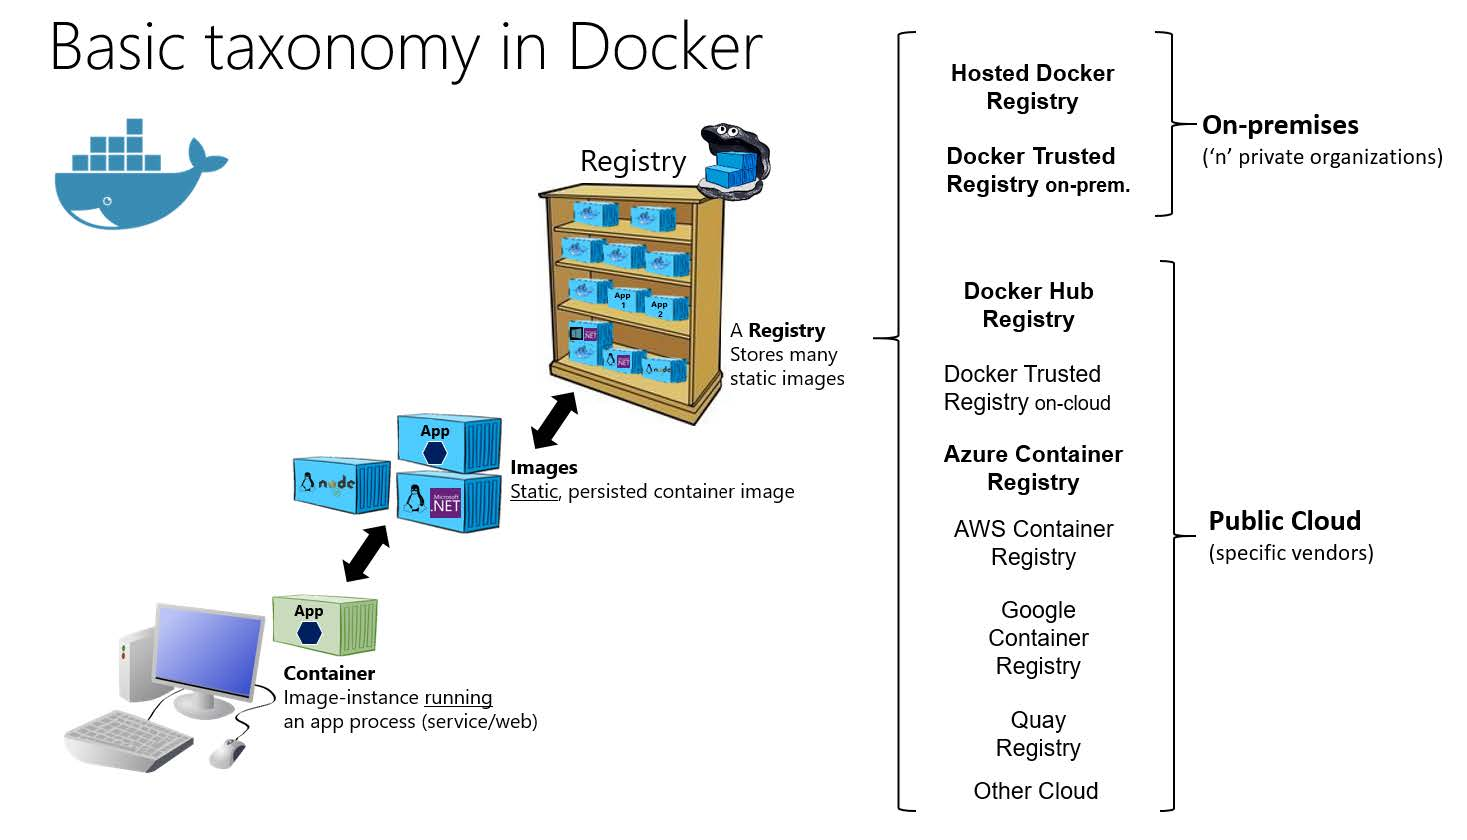
\includegraphics[width=1\textwidth]{imgs/1.1.jpg}}
    \caption*{\textit{Basic taxonomy in Docker, \href{https://docs.microsoft.com/ru-ru/dotnet/architecture/microservices/container-docker-introduction/docker-containers-images-registries}{Контейнеры, образы и реестры Docker}}\\}
    \label{1.1} %framework,fig1
\end{figure}


\subsubsection*{Контейнер (Container)}
\addcontentsline{toc}{subsubsection}{Контейнер (Container)}

Запущенный процесс или группу процессов в изолированном окружении принято называть
контейнером. Каждый такой контейнер — это уникальный объект. Он имеет свой идентификатор в
системе, и именно в нём происходит настоящая полезная работа. Отсюда и такое частое
употребление этого термина.\\


\subsubsection*{Образ контейнера (Container image)}
\addcontentsline{toc}{subsubsection}{Образ контейнера (Container image)}

Если же контейнер остановить, то всё, что от него останется, — это некоторый набор файлов на
файловой системе. И вот этот набор файлов, описывающих состояние остановленного контейнера,
называется образом контейнера или просто образом. Причём в зависимости от используемой
системы управления контейнерами набор файлов и их особенности могут различаться — это
задаётся форматом образа контейнера.

Сейчас \href{https://github.com/opencontainers/image-spec}{OCI-образ} — это наиболее популярный формат. В частности, актуальные версии Docker
используют именно этот формат образов. Что интересно, формат OCI-образа не зависит ни от
архитектуры процессора хозяйской системы, ни от используемой операционной системы в том
смысле, что этот формат может описать полное состояние контейнера на любой системе. Однако,
разумеется, один и тот же образ невозможно использовать на процессорах разных архитектур или в
хозяйских системах с разными ОС. Нюанс может заключаться в том, что контейнеры могут
запускаться внутри виртуальной машины и тем самым может создаваться видимость запуска
Linux-контейнера в Windows и наоборот.\\


\subsubsection*{Базовый образ (Base image)}
\addcontentsline{toc}{subsubsection}{Базовый образ (Base image)}

Как правило, контейнер создаётся не с нуля (это возможно, но используется редко), а из заранее
подготовленного образа. Причём этот образ, в сущности, — зафиксированное состояние ранее
использованного контейнера. То есть такие образы можно создавать, интерактивно делая изменения
в текущем контейнере. Однако чаще образы создают при помощи специального инструментария:
\href{https://docs.docker.com/engine/reference/builder/}{Docker и Dockerfile}, \href{https://buildah.io/}{Buildah} и т. д. Такие образы называют базовыми, так как используют их как базу
для своего продукта. Самый простой пример — это минимальная файловая система какого-нибудь
популярного Linux-дистрибутива, например Ubuntu, Alpine и т. д.\\


\subsubsection*{Реестр (Registry)}
\addcontentsline{toc}{subsubsection}{Реестр (Registry)}

Подготовленные образы можно хранить и использовать локально, но хорошая практика состоит в
публикации образов в соответствующих реестрах. Реестр образов — это некое подобие библиотеки, в
которой хранятся образы. Причём реестры используются не только и не столько для хранения
образов. Имея информацию о содержимом образа, а ещё лучше — использованный для его создания
Makefile, Dockerfile или shell-скрипт, можно запросто воссоздать образ самостоятельно. Реестры
нужны также для обмена образами и их распространения.

Наиболее известный на сегодняшний день реестр — это \href{https://hub.docker.com/}{Docker Hub}. Там можно найти образы
большинства популярных Linux-дистрибутивов, а также массу производных от них. Более того, любой
желающий может опубликовать самостоятельно подготовленный образ. К сожалению, найти
актуальную статистику по использованию Docker Hub весьма непросто, однако можно обратиться к
обзору из \href{https://habr.com/ru/company/flant/blog/337448/}{статьи на Habr.com}.

Существует и масса других реестров, начиная с публичных (\href{https://registry.fedoraproject.org/}{Fedora Container Registry}, \href{https://quay.io/}{Red Hat Quay}) и
заканчивая корпоративными или личными.\\


\subsubsection*{Среда исполнения контейнеров (Container runtime)}
\addcontentsline{toc}{subsubsection}{Среда исполнения контейнеров (Container runtime)}

Выше мы определили контейнер как набор процессов, запущенных в изоляции от хозяйской системы.
И образ контейнера как набор файлов, описывающих статическое состояние контейнера, когда он
остановлен. Соответственно, для воссоздания работающего контейнера из образа необходимо:

\begin{itemize}
    \item в соответствии с форматом образа прочитать из него информацию о конфигурации
    изолированной среды для запуска контейнера;
    \item прочитать файловую систему контейнера;
    \item создать и запустить необходимые процессы внутри изолированного окружения.
\end{itemize}

Перечисленный набор операций выполняет низкоуровневая среда исполнения контейнеров. Container
runtime — это некая аналогия среды выполнения вроде Java Runtime Environment (JRE), необходимая
для запуска байт-кода Java. Разница в том, что container runtime только создаёт необходимое
окружение и управляет жизненным циклом контейнера, а приложения или скрипты внутри контейнера
исполняются точно так же, как и приложения хозяйской системы без использования
runtime-окружения. Причём одной только среды исполнения контейнеров вполне достаточно для
создания и использования контейнеров. Типичный пример — runC.

\href{https://github.com/opencontainers/runc}{runC} — утилита командной строки, предназначенная для создания и запуска контейнеров в
соответствии со спецификацией Open Container Initiative (OCI).

Помимо runC, написанного почти полностью на Go, существует \href{https://github.com/containers/crun}{crun}. Это тоже Container Runtime,
реализующий спецификации OCI, но написанный на чистом Си. По сравнению с runC имеет более
высокую производительность и использует меньший объём памяти хозяйской системы при работе.\\


\subsubsection*{Container engine}
\addcontentsline{toc}{subsubsection}{Container engine}

Для упрощения работы с контейнерами функционал container runtime зачастую существенно
расширяется добавлением API удалённого управления, утилитами работы с образами контейнеров и
даже средствами удобного обмена образами и контейнерами. Такие комбайны принято называть
высокоуровневыми средствами для работы с контейнерами или container engine. В качестве примера
можно привести containerd или \href{https://podman.io/}{podman}.

В какую же категорию отнести Docker, мы узнаем позже, когда будем говорить именно о нём, а пока
просто примем к сведению, что Docker — это нечто большее.\\


\subsubsection*{Container engine}
\addcontentsline{toc}{subsubsection}{Container engine}


Первоначально идея виртуального окружения, впоследствии названного контейнером, сводилась к
запуску нескольких копий пользовательских пространств полноценной ОС на одной машине. Такие
контейнеры с полноценной ОС внутри принято называть системным контейнером или контейнером
операционной системы (ОС). Какое-то время системные контейнеры составляли серьёзную
конкуренцию полноценным виртуальным машинам, особенно на рынке веб-хостинга.\\


\subsubsection*{Контейнер приложения}
\addcontentsline{toc}{subsubsection}{Контейнер приложения}

Постепенно пришло понимание, что, имея уже одну полноценную ОС (имеется в виду хозяйская ОС),
нет необходимости запускать её копию со всеми десятками или сотнями служебных процессов, если
фактически необходимо запустить всего лишь одно приложение, например веб-сервер. Так появились
контейнеры приложений, которые содержат всё необходимое для запуска одного или нескольких
приложений или сервисов, а не полноценной ОС. Они занимают меньше места на диске и в памяти,
потребляют меньше ресурсов процессора хозяйской системы и позволяют реализовать ставшую
сейчас чрезвычайно популярной микросервисную архитектуру.

\href{https://ru.wikipedia.org/wiki/Ìèêðîñåðâèñíàÿ_àðõèòåêòóðà}{Микросервисная архитектура} — вариант сервис-ориентированной архитектуры программного
обеспечения, ориентированный на взаимодействие насколько это возможно небольших, слабо
связанных и легко изменяемых модулей — микросервисов. Получил распространение в середине
2010-х годов в связи с развитием практик гибкой разработки и DevOps.

Может даже оказаться, что контейнеры приложений гораздо более популярны, чем их системные
предки.\\


\subsection*{В Linux}
\addcontentsline{toc}{subsection}{В Linux}

Изоляция и управление группой процессов в Linux реализуются благодаря cgroups и namespaces.

\href{https://ru.wikipedia.org/wiki/Ïðîñòðàíñòâî_èì¸í_(Linux)}{Пространство имён} (англ. namespaces) — это функция ядра Linux, позволяющая изолировать и
виртуализировать глобальные системные ресурсы множества процессов.

При помощи namespaces происходит виртуализация или изоляция самых разнообразных ресурсов. А
cgroups позволяют эти виртуализированные ресурсы делать доступными только некоторым
процессам или группам (иерархиям или деревьям) процессов, а кроме того, управлять объёмом
доступных ресурсов. Точнее, вводить ограничения на их использование. И современные инструменты
контейнеризации в Linux построены с использованием упомянутых выше двух механизмов ядра.

Если сильно упростить, Docker, LXC, \href{https://en.wikipedia.org/wiki/Lmctfy}{lmctfy} или runC — это набор скриптов, которые самостоятельно
настраивают namespaces и cgroups, а после этого запускают указанное приложение в только что
созданном контейнере.


\subsubsection*{Cgroups}
\addcontentsline{toc}{subsubsection}{Cgroups}

\href{https://ru.wikipedia.org/wiki/Êîíòðîëüíàÿ_ãðóïïà_(Linux)}{Контрольная группа} (англ. control group, cgroups, cgroup) — группа процессов в Linux, для которой
механизмами ядра наложена изоляция и установлены ограничения на некоторые вычислительные
ресурсы: процессорные, сетевые, ресурсы памяти, ресурсы ввода-вывода. Механизм позволяет
образовывать иерархические группы процессов с заданными ресурсными свойствами и обеспечивает
программное управление ими. Следующие типы ресурсов хозяйской системы могут быть
использованы с cgroups:

\begin{enumerate}
    \item \textbf{CPU} — управляет распределением вычислительных ресурсов центрального процессора. Для
    каждой группы можно выделить часть процессорного времени ЦП, причём можно указывать
    либо относительное значение, например 30%, либо длительность периода учёта и
    длительность временного интервала, доступного для работы группы. Можно указать даже
    приоритет конкретной группы относительно других групп.
    \item \textbf{Memory} — управляет распределением памяти, позволяя процессам в данной группе
    использовать ограниченный объём памяти. Если процессы группы попытаются превысить
    максимально допустимое значение, они будут уничтожены при помощи механизма OOM killer.
    Это механизм в ядре ОС Linux, позволяющий в случае критического недостатка памяти для
    работы системы освободить место в ОЗУ за счёт уничтожения некоторых работающих
    процессов.
    \item \textbf{IO} — управляет распределением ресурсов подсистем ввода-вывода. Возможно ограничение
    либо по объёму прочитанных или записанных данных за единицу времени, либо по количеству
    операций ввода-вывода (IOPS) также за единицу времени.

    \href{https://ru.wikipedia.org/wiki/IOPS}{IOPS} (аббревиатура от англ. input/output operations per second — «количество операций ввода-вывода
в секунду»; произносится как «ай-опс») — количество операций ввода-вывода, выполняемых
системой хранения данных за одну секунду. Один из параметров, используемых для сравнения
систем хранения данных: жёстких дисков (НЖМД), твердотельных накопителей (SSD), сетевых
хранилищ SAN, NAS) и оценки их производительности.

    \item \textbf{PID} — управляет возможностью процессов группы создавать новые (дочерние) процессы.
    \item \textbf{Device controller} — управляет доступом процессов из группы к файлам устройств, обычно
    расположенным в папке /dev/. Возможно задание ограничений не только на создание новых
    файлов устройств, но также на доступ к уже имеющимся.
    \item \textbf{RDMA} — управляет доступом к RDMA-ресурсам.
    
    \href{https://ru.wikipedia.org/wiki/%D0%A3%D0%B4%D0%B0%D0%BB%D1%91%D0%BD%D0%BD%D1%8B%D0%B9_%D0%BF%D1%80%D1%8F%D0%BC%D0%BE%D0%B9_%D0%B4%D0%BE%D1%81%D1%82%D1%83%D0%BF_%D0%BA_%D0%BF%D0%B0%D0%BC%D1%8F%D1%82%D0%B8}{Удалённый прямой доступ к памяти} (англ. remote direct memory access, RDMA) — аппаратное
решение для обеспечения прямого доступа к оперативной памяти другого компьютера при помощи
высокоскоростной сети. Такой доступ позволяет получить доступ к данным, хранящимся в удалённой
системе, без привлечения средств операционных систем обоих компьютеров. Это метод пересылки
данных с высокой пропускной способностью и низкой задержкой сигнала, который особенно полезен в
больших параллельных вычислительных системах — кластерах.

    \item \textbf{Perf\_events} — управляет доступом к информации, предоставляемой подсистемой Perf ядра Linux.

    \href{https://en.wikipedia.org/wiki/Perf_(Linux)}{Perf} — средство оценки производительности разных систем ядра ОС, приложений пользователя,
аппаратуры и т. д. В основе этого инструмента лежит сбор разнообразной статистической
информации с возможным последующим её анализом.

\begin{figure}[h]%current location
    \centering
    \scalebox{0.7}{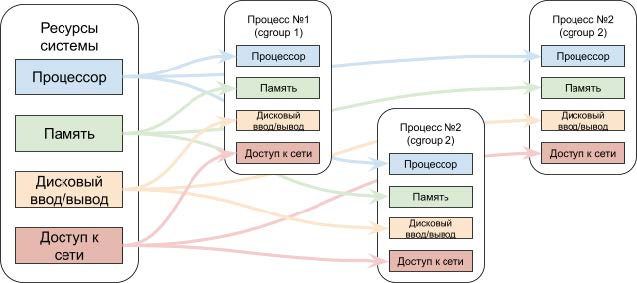
\includegraphics[width=1\textwidth]{imgs/1.2.jpg}}
    \caption*{\textit{Cgroups: управление ресурсами системы, предоставляемыми процессам пользователя}\\}
    \label{1.2}
\end{figure}

\end{enumerate}

\subsubsection*{Namespaces}
\addcontentsline{toc}{subsubsection}{Namespaces}

Пространства имён (namespaces) — это функциональная особенность ядра ОС Linux, благодаря
которой разные процессы в пространстве пользователя видят разные ресурсы так, как если бы они
были одними и теми же. То есть фактически ОС подменяет реальные свойства своих ресурсов при
предоставлении их пользовательским приложениям.

Например, мы знаем, что каждый процесс, запущенный поверх ядра Linux, должен иметь свой
уникальный идентификатор — Process ID (PID), назначенный ядром при создании данного процесса.
Благодаря namespaces можно сделать так, чтобы процесс считал, что его PID, например, равен 1, что
может быть только у первого пользовательского процесса в системе. В большинстве случаев это
процесс инициализации, то есть сегодня это обычно systemd.

Более того, дочерние процессы также будут видеть PID своего родителя, равный 1. При этом,
разумеется, реальный PID этого процесса, известный только ядру ОС и используемый ядром для
управления процессом, будет значительно отличаться от 1. Например, он будет 12345.

\begin{figure}[h]%current location
    \centering
    \scalebox{0.6}{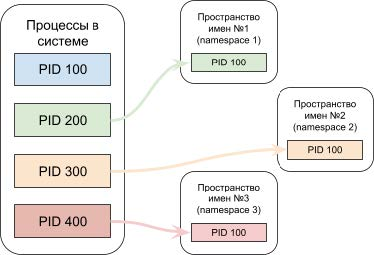
\includegraphics[width=1\textwidth]{imgs/1.3.jpg}}
    \caption*{\textit{PID namespace}}
    \label{1.3}
\end{figure}

На сегодняшний день реализованы такие виды пространства имён:

\begin{enumerate}
    \item \textbf{Файловая система} (Mount, mnt) — позволяет предоставлять каждому процессу или группе
    процессов свой собственный экземпляр дерева файловой системы. Прообразом этого
    пространства имён послужила \href{https://ru.wikipedia.org/wiki/Chroot}{chroot} — операция изменения корневого каталога в
    Unix-подобных операционных системах.
    \item \textbf{ID процессов (PID)} — позволяет назначать ID процессов независимо в каждом пространстве
    имён. Таким образом, в разных пространствах имён могут быть процессы с одинаковыми в
    рамках этих пространств ID.
    \item \textbf{Сети (Network)} — позволяет виртуализировать сетевой стек. То есть каждое пространство
    имён будет иметь свой пул IP-адресов и портов, свои таблицы маршрутизации, файервол и так
    далее.
    \item \textbf{Межпроцессное взаимодействие (IPC)} — изолирует средства межпроцессного
    взаимодействия пространства имён, такие как совместно используемая память, очереди
    сообщений, семафоры. Процессы из разных пространств не будут иметь возможности
    умышленно или неумышленно взаимодействовать друг с другом.
    \item \textbf{Пользовательские ID (User)}. Так же, как ID процессов, можно виртуализовать ID
    пользователей. User ID namespace позволяет сделать именно это: иметь одинаковые UID в
    разных пространствах имён.
    \item \textbf{Control group (cgroup)} — виртуализует cgroups.
    \item \textbf{UTS} — виртуализует имя хоста (hostname)\\
\end{enumerate}

\subsection*{В Windows}
\addcontentsline{toc}{subsection}{В Windows}

Изначально контейнеры в том виде, в каком мы их знаем сейчас, появились в UNIX-подобных ОС
(BSD, Linux). Но благодаря своей высокой популярности они нашли дорогу и в системы с ОС Windows.
Доступна \href{https://docs.microsoft.com/en-us/virtualization/windowscontainers/}{документация}, описывающая различные варианты реализации и использования
контейнеров в Windows.

Первоначально реализация контейнеров происходила путём запуска виртуальной машины с
обыкновенным или специализированным Linux-дистрибутивом. Позже компания Microsoft
реализовала решение, очень похожее на таковое в BSD и Linux, — изоляцию процессов без запуска
виртуальной машины. Кроме того, помимо похожей на BSD и Linux изоляции процессов средствами
ядра ОС, была реализована \href{https://docs.microsoft.com/en-us/archive/msdn-magazine/2017/april/containers-bringing-docker-to-windows-developers-with-windows-server-containers}{изоляция процессов средствами гипервизора Hyper-V}. Причём, несмотря
на то, что используется гипервизор Hyper-V, под его управлением запускается не полноценная и
независимая копия некой случайной ОС в том смысле, что это может быть любая ОС на выбор
пользователя, а клон уже работающей на хозяйской системе ОС. При этом переиспользуются её
части: файловая система, установленные приложения и прочее.

Имеется в виду переиспользование только тех частей ПО, которые доступны только для чтения. В
основном это исполняемый код, константы и строки. Если бы этот же набор ПО был заново
установлен в гостевую ОС, эти части ПО, доступные только для чтения, были бы точно такими же.
Изменяемые же части ПО, такие как данные пользователя, разумеется, не должны использоваться
совместно гостевой и хозяйской системами.

Таким образом, контейнерная революция добралась и до Windows. Однако стоит помнить о том, что в
отличие от виртуальных машин, как правило, не зависящих от хозяйской ОС или гипервизора,
контейнер полагается на базовые сервисы хозяйской ОС. А потому Linux-контейнер принципиально
невозможно запустить непосредственно на Windows и наоборот. Это становится возможным только в
случае использования виртуальной машины с запущенной в ней ОС необходимого типа.

В статье \href{https://docs.microsoft.com/en-us/virtualization/windowscontainers/deploy-containers/linux-containers.}{Linux containers on Windows 10} подробно рассматриваются доступные варианты запуска
Linux-контейнеров на Windows.

По сравнению с Linux-контейнерами их версия для Windows обладает \href{https://containerjournal.com/topics/container-ecosystems/why-windows-containers-are-less-attractive-than-linux-containers/}{определёнными недостатками}:

\begin{enumerate}
    \item \href{https://docs.microsoft.com/en-us/virtualization/windowscontainers/about/faq#what-are-the-prerequisites-for-running-containers-on-windows}{Не любая версия Windows подходит для запуска контейнеров}. Подойдут, например, Windows
    Server 2016 и Windows 10 Professional или Enterprise, начиная с Anniversary update (версия
    1607).
    \item \href{https://docs.microsoft.com/en-us/virtualization/windowscontainers/about/faq#how-are-containers-licensed-is-there-a-limit-to-the-number-of-containers-i-can-run}{Наличие ограничений, связанных с лицензированием}. Не на любой системе с Windows можно
    запустить неограниченное количество Windows-контейнеров.
    \item Гораздо меньшее количество реестров с образами Windows-контейнеров.\\
\end{enumerate}

\subsection*{В macOS}
\addcontentsline{toc}{subsection}{В macOS}

Ситуация с контейнерами в macOS примерно такая же, как в Windows. Разница лишь в том, что своей
собственной реализации окружения для запуска контейнеров непосредственно на macOS до сих пор
не было разработано. То есть использование контейнеров в macOS ограничивается запуском их в
виртуальной машине. До недавних пор всё сводилось к установке VMware Fusion или Oracle
VirtualBox, в них устанавливался полноценный Linux-дистрибутив. Далее задача становилась
тривиальной — запуск Linux-контейнеров в Linux. Позже в macOS был реализован собственный
фреймворк для создания легковесных гипервизоров — \href{https://developer.apple.com/documentation/hypervisor}{Hypervisor.framework}, ставший доступным,
начиная с macOS 10.10 Yosemite. Появилась возможность отказаться от полноценного внешнего
гипервизора и создать специализированный, нацеленный на обслуживание нужд контейнеризованных
окружений. Что и сделала компания Docker Inc., создав специально для macOS \href{https://github.com/moby/hyperkit}{инструмент под
названием HyperKit}.\newpage


\section*{Сравнение контейнеров и виртуальных машин}
\addcontentsline{toc}{section}{Сравнение контейнеров и виртуальных машин}

\subsection*{Производительность}
\addcontentsline{toc}{subsection}{Производительность}

Говоря о производительности, мы подразумеваем скорее обратное — накладные расходы на
обслуживание всей активности, не связанной напрямую с выполнением полезной работы гостевой
системой. И в этом смысле контейнеры имеют преимущества:

\begin{enumerate}
    \item Нет необходимости переключаться между режимами гипервизора и режимом работы гостевых
    систем. Это, как мы помним, достаточно накладная операция.
    \item Нет необходимости эмулировать аппаратуру, включая части центрального процессора, такие
    как MMU.
    \item Собственно сам гипервизор отсутствует в системе, а потому на его сервисные функции не
    приходится тратить процессорное время. Мы избавлены от ещё одного уровня абстракции,
    который, в отличие от контейнеров, очень часто оказывается реально исполняемым
    аппаратурой.
\end{enumerate}

Другими словами, контейнеры в общем случае \href{https://www.stratoscale.com/blog/data-center/running-containers-on-bare-metal}{позволяют более эффективно использовать
вычислительные ресурсы хозяйской системы}. Более высокая эффективность контейнеров
проявляется как минимум в двух важных аспектах:

\begin{enumerate}
    \item \textbf{Гораздо более быстрый старт полезной задачи}. Это особенно справедливо для
    контейнеров приложений, в которых после создания всего необходимого окружения
    необходимо запустить только целевое приложение, например веб-сервер. Контейнеры
    операционных систем, содержащие полный набор библиотек и приложений пользовательского
    пространства, стартуют медленнее, поскольку происходит запуск множества служб и
    сервисных процессов. Но даже при этом не происходит перезапуска ядра ОС и связанной с
    этим процессом инициализации аппаратуры, что само по себе может привносить
    существенные задержки.
    \item \textbf{Более высокая плотность размещения виртуализованных окружений на одной
    хозяйской машине}. Очевидно, что для запуска N копий веб-сервера в контейнерах
    приложений потребуется меньше ресурсов хозяйской системы, нежели для запуска N копий
    полноценных виртуальных машин с полными ОС и одним веб-сервером в каждой.
\end{enumerate}

Несмотря на высокую скорость работы ЦП, измеряемую в гигагерцах, и высокоскоростные шины
данных, такие как PCIe, при инициализации некоторого оборудования происходят задержки. Этому
может быть несколько причин. Зачастую внешнее оборудование имеет внутри свой процессор,
исполняющий код его же прошивки. Часто эта прошивка загружается во внешнее устройство с
хозяйской системы, причём иногда при помощи относительно низкоскоростного интерфейса типа SPI.
После того как прошивка была загружена, контроллер внешнего устройства начинает свою процедуру
инициализации. Только проверив все внутренние состояния, выполнив необходимые калибровки и
включив все свои устройства, он готов к взаимодействию с хозяйской системой.

Ещё хуже дело обстоит с инициализацией дисковых и сетевых устройств. Приводы с вращающимися
дисками должны раскрутить эти диски до рабочей скорости в тысячи оборотов в минуту, обычно до
5 400 или 7 200 об/мин. Разумеется, это не происходит мгновенно. А в случае сетевых устройств
согласование режима работы на физическом уровне, известное как autonegotiation, может занимать
буквально секунды.\\

\subsection*{Универсальность}
\addcontentsline{toc}{subsection}{Универсальность}

В плане универсальности контейнеры проигрывают полноценным виртуальным машинам, так как
контейнеры по определению используют ядро хозяйской ОС. Таким образом, невозможно запустить
контейнер, предназначенный для работы в Windows, Solaris или FreeBSD, на машине с
Linux-дистрибутивом. Современные же гипервизоры могут запускать гостевые системы с
разнообразными ОС: Windows, Linux, Solaris и т. д. Причём все эти гостевые системы отлично
уживается друг с другом.

Но даже при использовании гостевых систем одного типа, например Linux-дистрибутивов, в системе
контейнеризации принципиально невозможно иметь ядро ОС с разной функциональностью.
Безусловно, при помощи cgroups в Linux можно ограничить доступ процессов контейнера к
имеющейся функциональности хозяйского ядра ОС. Однако добавить дополнительную
функциональность ядра ОС для данного контейнера возможно, лишь изменив ядро хозяйской
системы. Что в свою очередь может потребовать перезапуска ядра, а это означает неминуемую
остановку всех контейнеров, запущенных в данной системе. В отдельно взятой виртуальной машине
можно производить любые изменения ядра ОС без опасения навредить процессам, запущенным в
соседних ВМ.\\

\subsection*{Безопасность}
\addcontentsline{toc}{subsection}{Безопасность}

Каждый производитель или разработчик нахваливает своё решение. Зачастую они используют не
слишком веские доводы или апеллируют к общим принципам, забывая о важных нюансах или
умышленно умалчивая о них.

Принято считать, что полноценная виртуализация позволяет обеспечить существенно более
надёжную изоляцию между гостевыми системами, нежели контейнеры. Основной довод, приводимый
апологетами данной позиции: благодаря совместно используемому ядру ОС, процесс, «убежавший»
из своего контейнера, может как минимум навредить всей системе в целом, помешав нормальной
работе ядра ОС. Или даже, получив доступ к данным, описывающим другие процессы в системе,
пробраться в соседний контейнер и выполнить в нём какие-то злонамеренные действия.

На первый взгляд, полноценные виртуальные машины лишены этого недостатка, так как
используемое гостевыми системами ПО полностью изолировано от других гостей. Но если взглянуть
на систему виртуализации более внимательно, то обнаружится гипервизор, управляющий всеми
гостевыми системами. То есть можно представить себе ситуацию, когда злонамеренный процесс
«совершит побег» из своей ВМ и проникнет в гипервизор благодаря уязвимости в коде гипервизора
или даже некоторым особенностям аппаратуры процессора.
newpage
К сожалению, это вовсе не теоретические рассуждения. Достаточно взглянуть на \href{https://en.wikipedia.org/wiki/Virtual_machine_escape}{неполный список
известных побегов из ВМ}, чтобы оценить масштабы бедствия. Разнообразные гипервизоры
оказываются жертвами, и проблема со временем никуда не девается. Более того, о многих
имеющихся до сих пор уязвимостях мы, простые пользователи и даже исследователи компьютерной
безопасности, ещё не знаем.

Таким образом, вопрос о более безопасном решении до сих пор остаётся открытым. Думается, что
более безопасной систему может сделать комплекс технологий и процессов, обеспечивающих
снижение рисков по всем возможным направлениям, а не попытка использовать лишь одну
«магическую» технологию.

Однако стоит отметить, что в реальной жизни контейнеры обычно запускаются внутри виртуальных
машин, которые заменяют собой физические машины. Так осуществляется высокая изоляция
контейнеров и сохраняется высокая эффективность использования ресурсов контейнерами.
Характерный пример — арендованный виртуальный сервер, на котором запущены разнообразные
сервисы, реализованные в контейнерах. В настоящее время обычно речь идёт о виртуальной машине
KVM.\newpage



\section*{Сравнение контейнеров и виртуальных машин}
\addcontentsline{toc}{section}{Сравнение контейнеров и виртуальных машин}

\subsection*{Безопасность}
\addcontentsline{toc}{subsection}{Безопасность}

Virtuozzo и OpenVZ (сокращение от Open Virtuozzo) — это продукты компании Parallels, позволяющие
на одной физической машине создавать множество виртуальных окружений (virtual environments). В
современной терминологии эти продукты можно было бы назвать контейнерами операционных
систем, так как упомянутые виртуальные окружения содержали внутри полноценные
Linux-дистрибутивы. Похоже, что даже термин Virtual Private Server (VPS) появился в своё время
благодаря Virtuozzo/OpenVZ.

Разработка Virtuozzo началась в прошлом тысячелетии, в 1999 году, если быть более точными. Его
разработали инженеры компании SWsoft, в 2007 году переименованной в Parallels, \href{https://openvz.livejournal.com/49158.html}{на основе ядра ОС
Linux версии 2.2}. А в январе 2002 года был выпущен первый коммерческий продукт — Virtuozzo 2.0, но
уже \href{https://cdn.kernel.org/pub/linux/kernel/v2.4/old-test-kernels/linux-2.4.0-test1.tar.gz}{на основе ядра Linux версии 2.4.0 test1}.

В 2005 году было принято решение открыть все наработки команды Parallels в ядре Linux, а также
необходимый минимум утилит управления. Так появился \href{https://www.linux.com/news/swsoft-offers-free-open-source-version-virtuozzo/}{проект OpenVZ}. Поскольку основой Virtuozzo
было ядро Linux, в тот момент не обладавшее средствами создания и управления виртуальными
окружениями, то все изменения относительно ванильного ядра приходилось адаптировать к новым
выпускам ядра Linux, которое весьма существенно изменяется от версии к версии. То есть только для
обновления версии используемого ядра Linux приходилось затрачивать существенные инженерные
ресурсы. Термин «контейнер» тогда ещё не был в ходу, он появился в названии продукта Solaris
Containers компании Sun Microsystems в январе 2005 года.

\href{https://ru.wikipedia.org/wiki/Âàíèëüíîå_ÿäðî}{Ванильное ядро} (vanilla kernel, mainline kernel) — термин, которым называют оригинальную версию
ядра Linux, в которую не было внесено изменений по сравнению с kernel.org. Вероятно, такое
значение («стандартный», «вариант по умолчанию») у слова «ванильный» появилось благодаря
популярности ванильного пломбира, который подразумевается по умолчанию, если речь идёт о самом
простом мороженом.


Решение этой проблемы состоит в интеграции своих изменений в основной код ядра. Благодаря
этому в более новых ядрах необходимый код уже будет присутствовать. Так наработки инженеров
Parallels оказали существенное влияние на развитие технологии Linux-контейнеров. В частности,
такие компоненты, как PID namespaces, network namespaces, memory cgroups, \href{https://criu.org/}{Checkpoint/Restore In
Userspace (CRIU)} и многие другие были либо разработаны, либо усовершенствованы инженерами
Parallels. Подробности можно узнать \href{https://wiki.openvz.org/FAQ#When_OpenVZ_will_be_in_upstream_kernel.3F}{в разделе FAQ проекта OpenVZ на «Википедии»}.

\begin{figure}[H]
    \centering
    \scalebox{0.5}{
\includegraphics[width=1\textwidth]{imgs/3.0.jpg}}
    \caption*{\textit{\href{https://www.slideshare.net/openvz/whats-missing-from-upstream-kernel-containers-kir-kolyshkin}{Количество изменённых строк кода в ядре Virtuozzo относительно ванильного ядра Linux}}}
    \label{3.0}
\end{figure}

Ниже вы видите график, иллюстрирующий количество изменений, сделанных инженерами компании
Parallels и принятых в основной код ядра Linux.

\begin{figure}[H]
    \centering
    \scalebox{1}{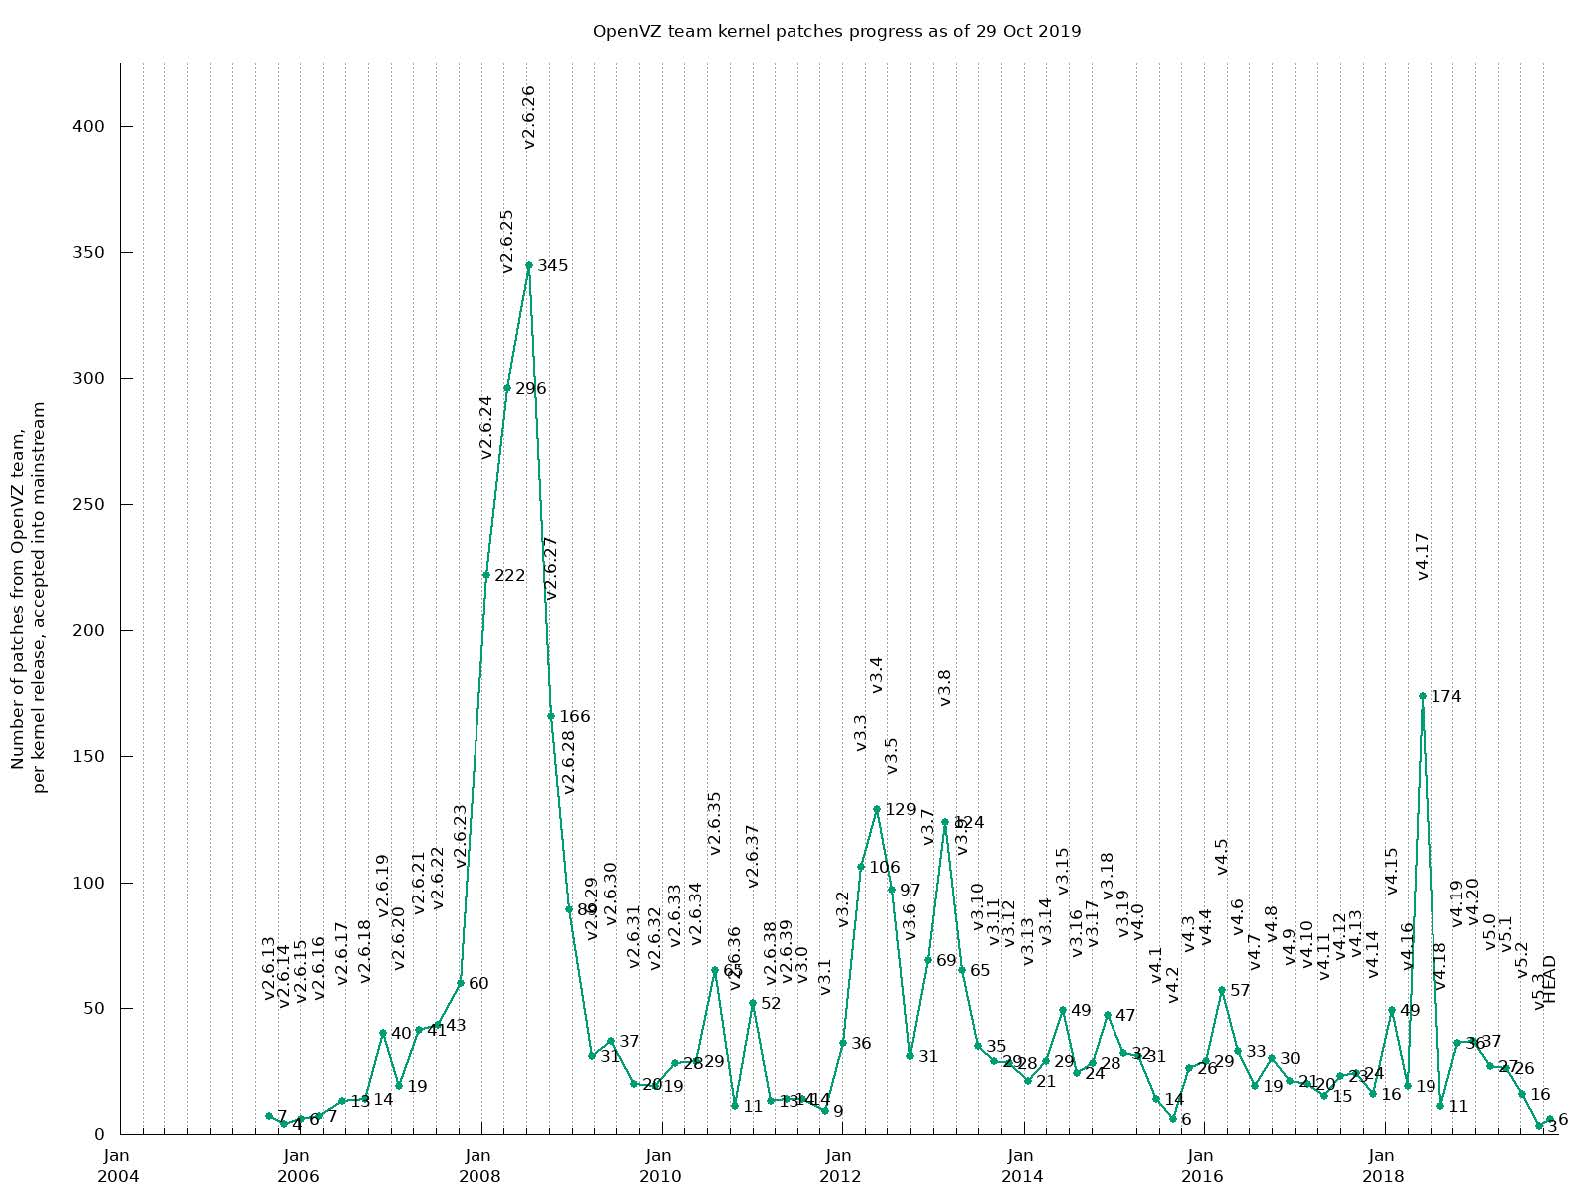
\includegraphics[width=1\textwidth]{imgs/3.1.jpg}}
    \label{3.1}
\end{figure}

Позже продукты OpenVZ и Virtuozzo \href{https://lists.openvz.org/pipermail/announce/2016-July/000664.html}{были объединены в продукт}, взявший имя открытого проекта
OpenVZ.

В настоящее время разработка OpenVZ, похоже, сводится к выпуску минорных версий ядра из
состава Red Hat Enterprise Linux 6 для OpenVZ 6. Решения на базе OpenVZ/Virtuozzo можно найти
лишь в давно используемых системах, которые ещё не были или уже никогда и не будут переведены
на использование более современных технологий. Тем не менее, благодаря успешным продуктам для
создания виртуальных окружений, появились и существенно развились удобные, безопасные и
эффективные инструменты для создания контейнеров и управления ими.

Интересно отметить, что OpenVZ/Virtuozzo в основном нашли применение на рынке хостинга
веб-сайтов, где долгое время невероятно популярный VPS-хостинг был синонимом OpenVZ/Vituozzo.
Так произошло во многом благодаря низкой стоимости, которая стала возможной благодаря запуску
множества виртуальных окружений на одном физическом сервере. Однако с появлением более
мощных серверов и удобной и эффективной виртуализации на базе KVM всё больше
хостинг-провайдеров стали переходить на предоставление клиентам экземпляров виртуальных
машин вместо контейнеров. Видя спрос на решения на базе KVM, компания Parallels в последнем
релизе OpenVZ добавила поддержку управления виртуальными машинами поверх гипервизора KVM.

Тем самым она сделала OpenVZ универсальным инструментом для управления виртуальными
окружениями обоих типов: контейнерами и полноценными виртуальными машинами.\\

\subsection*{LXC и LXD}
\addcontentsline{toc}{subsection}{LXC и LXD}

Именно благодаря наработкам в ядре Linux, сделанным для OpenVZ/Virtuozzo, стало возможным
появление нового инструментария для создания контейнеров и управления ими. Он был назван
незамысловато — Linux Containers, сокращённо LXC. Интересно, что в отличие от OpenVZ/Virtuozzo,
LXC использует функциональность ванильного ядра Linux без каких-либо дополнительных изменений,
а потому позволяет использовать практически любой современный Linux-дистрибутив для создания
или запуска соответствующих контейнеров. Как и его предшественники (парочка OpenVZ/Virtuozzo),
LXC создаёт виртуальное окружение, предназначенное для запуска полноценной ОС, — разумеется,
лишь его часть в пространстве пользователя, без ядра ОС. По сути, LXC можно было бы назвать
примерной реализацией системных контейнеров в Linux.

Пошаговую инструкцию для начинающих можно найти на \href{https://linuxcontainers.org/ru/lxc/getting-started/}{сайте Linux Containers}. Важно отметить, что,
будучи достаточно низкоуровневым инструментарием, LXC требует выполнения пользователем
относительно большого количества настроек хозяйской системы по сравнению с инструментами,
которые будут рассмотрены позже. Но есть в этом и красота инструментария в духе UNIX: простые
утилиты хорошо выполняют простой набор операций, а более сложные задачи решаются путём
запуска разных утилит пользователем.

Поскольку работа с низкоуровневыми утилитами не всегда удобна, особенно при использовании
множества контейнеров и сложных сценариях управления, спустя некоторое время был разработан
новый, более высокоуровневый, инструментарий — LXD. Читается «лекс-ди», это сокращение от
Linux Container Daemon. Его разработчики, в основном инженеры компании Canonical, называют LXD
гипервизором контейнеров, делая отсылку к диспетчеру виртуальных машин, также именуемому
гипервизором. Хотя, разумеется, никакой это не гипервизор, а просто диспетчер контейнеров.

В случае диспетчера виртуальных машин название «гипервизор» вполне уместно, так как оно
противопоставляется «супервизору», в качестве которого выступает ядро ОС. И гипервизор
оказывается как бы супервизором супервизоров, отсюда и «гипер-». 
При использовании контейнеров диспетчер контейнеризованных окружений не управляет
супервизорами этих окружений, потому как все эти окружения используют ядро хозяйской системы,
поверх которого работает и сам диспетчер. Так что «гипервизор контейнеров» — это в определённом
смысле преувеличение или метафора.

Ещё более ёмко и точно LXD описывается в \href{https://github.com/lxc/lxd}{GitHub-репозитории}, где ведётся его разработка: «демон,
использующий liblxc и предоставляющий REST API для управления контейнерами». Кроме демона,
который управляет непосредственно контейнерами, разрабатывают и удобный клиент для простого
взаимодействия с демоном. Доля иронии заключается в том, что клиент для lxd носит название lxc,
хотя его последняя буква — сокращение от client, а не container.

Благодаря такой клиент-серверной архитектуре возможно удалённое управление демоном, то есть
совсем не обязательно запускать клиент управления на той же машине, что и демон. Это сделало
возможным создание клиентов в том числе для \href{https://chocolatey.org/packages/lxc}{ОС Windows} и даже \href{https://chocolatey.org/packages/lxc}{macOS}.

Хочется надеяться, что мы помогли вам разобраться, чем же различаются LXC и LXD. Тем не менее
рекомендуем начать своё знакомство с Linux Containers именно с LXD. Это более удобный и простой в
освоении инструментарий. Инструкции для начала работы с LXD, в том числе и на русском языке,
\href{https://linuxcontainers.org/ru/lxd/getting-started-cli/}{доступны на официальном сайте проекта}.

Более того, можно воспользоваться \href{https://linuxcontainers.org/lxd/try-it/}{облачным сервисом проекта} и получить опыт работы с LXD без
подготовки своей собственной системы.

Имея хозяйскую систему с дистрибутивом Ubuntu 16.04, запустим контейнер с CentOS 7:

\begin{lstlisting}
root@tryit-welcomed:~# lxc launch images:centos/7 centos-7
root@tryit-welcomed:~# lxc exec centos-7 -- /bin/bash
\end{lstlisting}

И можем наблюдать следующее внутри контейнера:\\
\begin{lstlisting}
[root@centos-7 ~]# ps -aef --forest
UID        PID  PPID  C STIME TTY          TIME CMD
root       316     0  0 20:35 ?        00:00:00 /bin/bash
root       338   316  0 20:41 ?        00:00:00  \_ ps -aef --forest
root         1     0  0 20:35 ?        00:00:00 /sbin/init
root        35     1  0 20:35 ?        00:00:00 /usr/lib/systemd/systemd-journald
root        36     1  0 20:35 ?        00:00:00 /usr/lib/systemd/systemd-udevd
root        58     1  0 20:35 ?        00:00:00 /usr/lib/systemd/systemd-logind
dbus        59     1  0 20:35 ?        00:00:00 /usr/bin/dbus-daemon --system --address=systemd: --nofork --nopidfile --systemd-activation
root        71     1  0 20:35 console  00:00:00 /sbin/agetty --noclear --keep-baud console 115200,38400,9600 linux
root        72     1  0 20:35 ?        00:00:00 /usr/sbin/crond -n
root       250     1  0 20:35 ?        00:00:00 /sbin/dhclient -1 -q -lf /var/lib/dhclient/dhclient--eth0.lease -pf /var/run/dhclient-eth0.pid -H cento 
root       311     1  0 20:35 ?        00:00:00 /usr/sbin/rsyslogd -n
\end{lstlisting}

Вывод утилиты ps — она отображает запущенные в системе процессы — стоит запомнить для
сравнения с тем, что мы увидим при использовании контейнеров приложений:

\begin{lstlisting}
[root@centos-7 ~]# cat /etc/centos-release
CentOS Linux release 7.7.1908 (Core)
[root@centos-7 ~]# uname -r -v
4.4.0-170-generic #199-Ubuntu SMP Thu Nov 14 01:45:04 UTC 2019
\end{lstlisting}

Также интересно обратить внимание на содержимое файла /etc/centos-release и даже сам факт его
наличия. Сравните его с полным названием версии ядра ОС. Легко обнаружить, что запущен
дистрибутив CentOS версии 7.7, однако ядро ОС вовсе не из этого дистрибутива, а из хозяйской
системы с Ubuntu 16.04. Linux-дистрибутив CentOS 7, как и его двойник Red Hat Enterprise Linux 7,
использует ядро Linux версии 3.10.

Интересные особенности LXC/LXD:
\begin{enumerate}
    \item Наличие \href{https://images.linuxcontainers.org/}{реестра заранее подготовленных образов} почти всех популярных дистрибутивов.
    Запуск нового контейнера производится быстро и просто: как мы видели в примере выше,
    достаточно всего двух команд.
    \item Если LXC как низкоуровневый инструментарий для создания контейнеров и управления ими
    доступен в любом современном Linux-дистрибутиве, то LXD — в каком-то смысле удобная
    надстройка над LXC — в основном доступен в Ubuntu. Это не удивительно, так как в основном
    именно инженеры Canonical занимаются разработкой LXD. Однако благодаря системе
    управления пакетами Snappy LXD возможно установить и в прочих дистрибутивах.
\end{enumerate}

\href{https://ru.wikipedia.org/wiki/Snappy_(%D1%81%D0%B8%D1%81%D1%82%D0%B5%D0%BC%D0%B0_%D1%83%D0%BF%D1%80%D0%B0%D0%B2%D0%BB%D0%B5%D0%BD%D0%B8%D1%8F_%D0%BF%D0%B0%D0%BA%D0%B5%D1%82%D0%B0%D0%BC%D0%B8))}{Snappy} — система развёртки и управления пакетами, также разработанная Canonical для мобильной
Ubuntu. Инструкция по установке snapd (собственно, диспетчера пакетов Snappy) \href{https://snapcraft.io/docs/installing-snapd}{доступна на сайте
snapcraft.io}. Однако стоит понимать, что пакеты Snappy, будучи сторонними по отношению к своей
системе управления пакетами дистрибутивов, отличных от Ubuntu, могут давать несколько
неожиданный результат. Мы не говорим о производных от Ubuntu вроде Mint и прочих.

\begin{enumerate}
    \item [3.]LXC — это набор утилит, а LXD — это в первую очередь демон, использующий liblxc, то есть,
    по сути, набор инструментария LXC. Не путайте с клиентом LXD под названием lxc.
    \item [4.]Будучи полноценным Linux-дистрибутивом, LXC-контейнеры позволяют запускать контейнеры
    внутри себя, тем самым реализуя вложенную контейнеризацию. Не то чтобы это где-то
    широко использовалось, но сама по себе возможность есть. Для сравнения, контейнеры
    приложений, которые мы рассмотрим в дальнейшем, на такое принципиально не способны.
    \item [5.]В \href{https://discuss.linuxcontainers.org/t/lxd-3-18-has-been-released/5869}{LXD версии 3.18}, выпущенном в октябре 2019 года, \href{https://github.com/lxc/lxd/issues/6205}{разработчики заявили о поддержке не
    только LXC-контейнеров, но также и полноценных виртуальных машин}. Можно будет выбирать
    тип изоляции (контейнер или виртуальная машина) передачей одного параметра при
    использовании стандартного клиента lxc или при использовании непосредственно REST API,
    предоставляемого демоном LXD.
\end{enumerate}

Забавно наблюдать повторение пути, пройденного инженерами компании Parallels. Мы помним, как их
продукт OpenVZ 7.0, объявленный в далёком уже 2016 году, преподносился как универсальное
решение для виртуализации. На выбор пользователя предлагалось использование виртуального
окружения Virtuozzo или полноценной ВМ на основе KVM.\\


\subsection*{Docker}
\addcontentsline{toc}{subsection}{Docker}

Мы поговорили о LXC и LXD как о правильно реализованной технологии Linux-контейнеров в их
первоначальном смысле — как о виртуализованном дистрибутиве, изолированном от хозяйской
системы и себе подобных. Имеется в виду использование только той функциональности, которую
предоставляет ванильное ядро, без «секретного соуса» отдельных разработчиков или компаний.
Теперь стоит познакомиться с Docker.

\href{https://www.youtube.com/watch?v=wW9CAH9nSLs}{Первое упоминание Docker}, продукта компании dotCloud, прозвучало в выступлении основателя
Docker Inc. (в тот момент ещё dotCloud Inc.) Соломона Хайкса на конференции PyCon 2013.

На сегодняшний день Docker — практически синоним почти всего, что связано с контейнерами. По
крайней мере, у обывателя может возникнуть такое ощущение. Хотя в конце 2019 года при более
внимательном взгляде становится понятно, что помимо Docker существует ещё множество продуктов
и решений, которые серьёзно угрожают компании Docker Inc. и их продуктам. Подробнее об этом вы
можете прочитать в статьях \href{http://crunchtools.com/why-no-docker/?preview=true&frame-nonce=388d01a716}{Part II: Why Is There No Docker in OpenShift 4 and RHEL 8?} и \href{https://www.mirantis.com/blog/mirantis-acquires-docker-enterprise-platform-business/}{What We
Announced Today and Why it Matters} (Mirantis приобретает Docker Enterprise platform у Docker Inc.).

Так что же такое Docker? Первое, с чем стоит определиться: Docker Inc. — это компания,
занимающаяся разработкой одноимённого продукта. Продукты компании Docker Inc. — это средства
для создания и распространения контейнеров, а также управления ими. В частности, Docker Engine,
Docker Compose, Docker Desktop for Mac/Windows, в конце концов, Docker Hub.

Отметим, что Docker Engine до версии 0.9 использовал LXC, инструменты которого в основном
реализованы на языке Си, \href{https://www.docker.com/blog/docker-0-9-introducing-execution-drivers-and-libcontainer}{как средство создания и запуска контейнеров}. Начиная с версии 0.9,
Docker использует свой движок libcontainer, полностью написанный на языке программирования Go.
Более того, Docker Engine первоначально представлял собой один исполняемый файл /usr/bin/docker,
который содержал функциональность демона, клиента, средства построения контейнеров, а также
клиента для работы с реестрами образов. Так было проще разрабатывать и распространять ещё не
очень сложный программный продукт.

Существенные изменения произошли в версии 1.11. Во-первых, разработчики разделили клиента и
демона, теперь это стал /usr/bin/dockerd. Более того, уже в версии 1.12 были вынесены в отдельные
модули \href{https://github.com/opencontainers/runc}{среды исполнения контейнеров runC} и \href{https://github.com/docker-archive/containerd}{низкоуровневый инструмент для взаимодействия с
абстрактной средой исполнения контейнеров containerd}.

И чем дальше, тем больше происходит разделение ранее монолитного инструмента на множество
модулей. Причём в соответствии со своим \href{https://www.docker.com/blog/runc/}{Infrastructure Plumbing Manifesto} компания Docker будет
стараться:
\begin{enumerate}
    \item Всегда, если это возможно, повторно использовать уже имеющиеся компоненты и отдавать
    назад свои улучшения. Если же действительно необходимо создать новый компонент, то
    делать его лёгким в повторном использовании и предусмотреть возможность принятия
    улучшений от сторонних разработчиков.
    \item Следовать принципам UNIX: несколько простых компонентов лучше, чем один, но сложный.
    \item Определять стандартные интерфейсы, которые позволят с лёгкостью связать несколько
    простых компонентов в одну сложную систему.
\end{enumerate}

Сегодня мы видим результаты следования этим принципам: инструментарий Docker стал глубоко
модульным, что даёт возможность использовать только те его части и в том виде, который наиболее
удовлетворяет требованиям конкретного случая. Апофеоз этой модульной структуры — \href{https://mobyproject.org/}{проект Moby}.
При помощи Moby, как из кирпичиков Lego, можно построить как Docker, так и свою собственную
систему управления контейнерами.

\begin{figure}[H]
    \centering
    \scalebox{0.9}{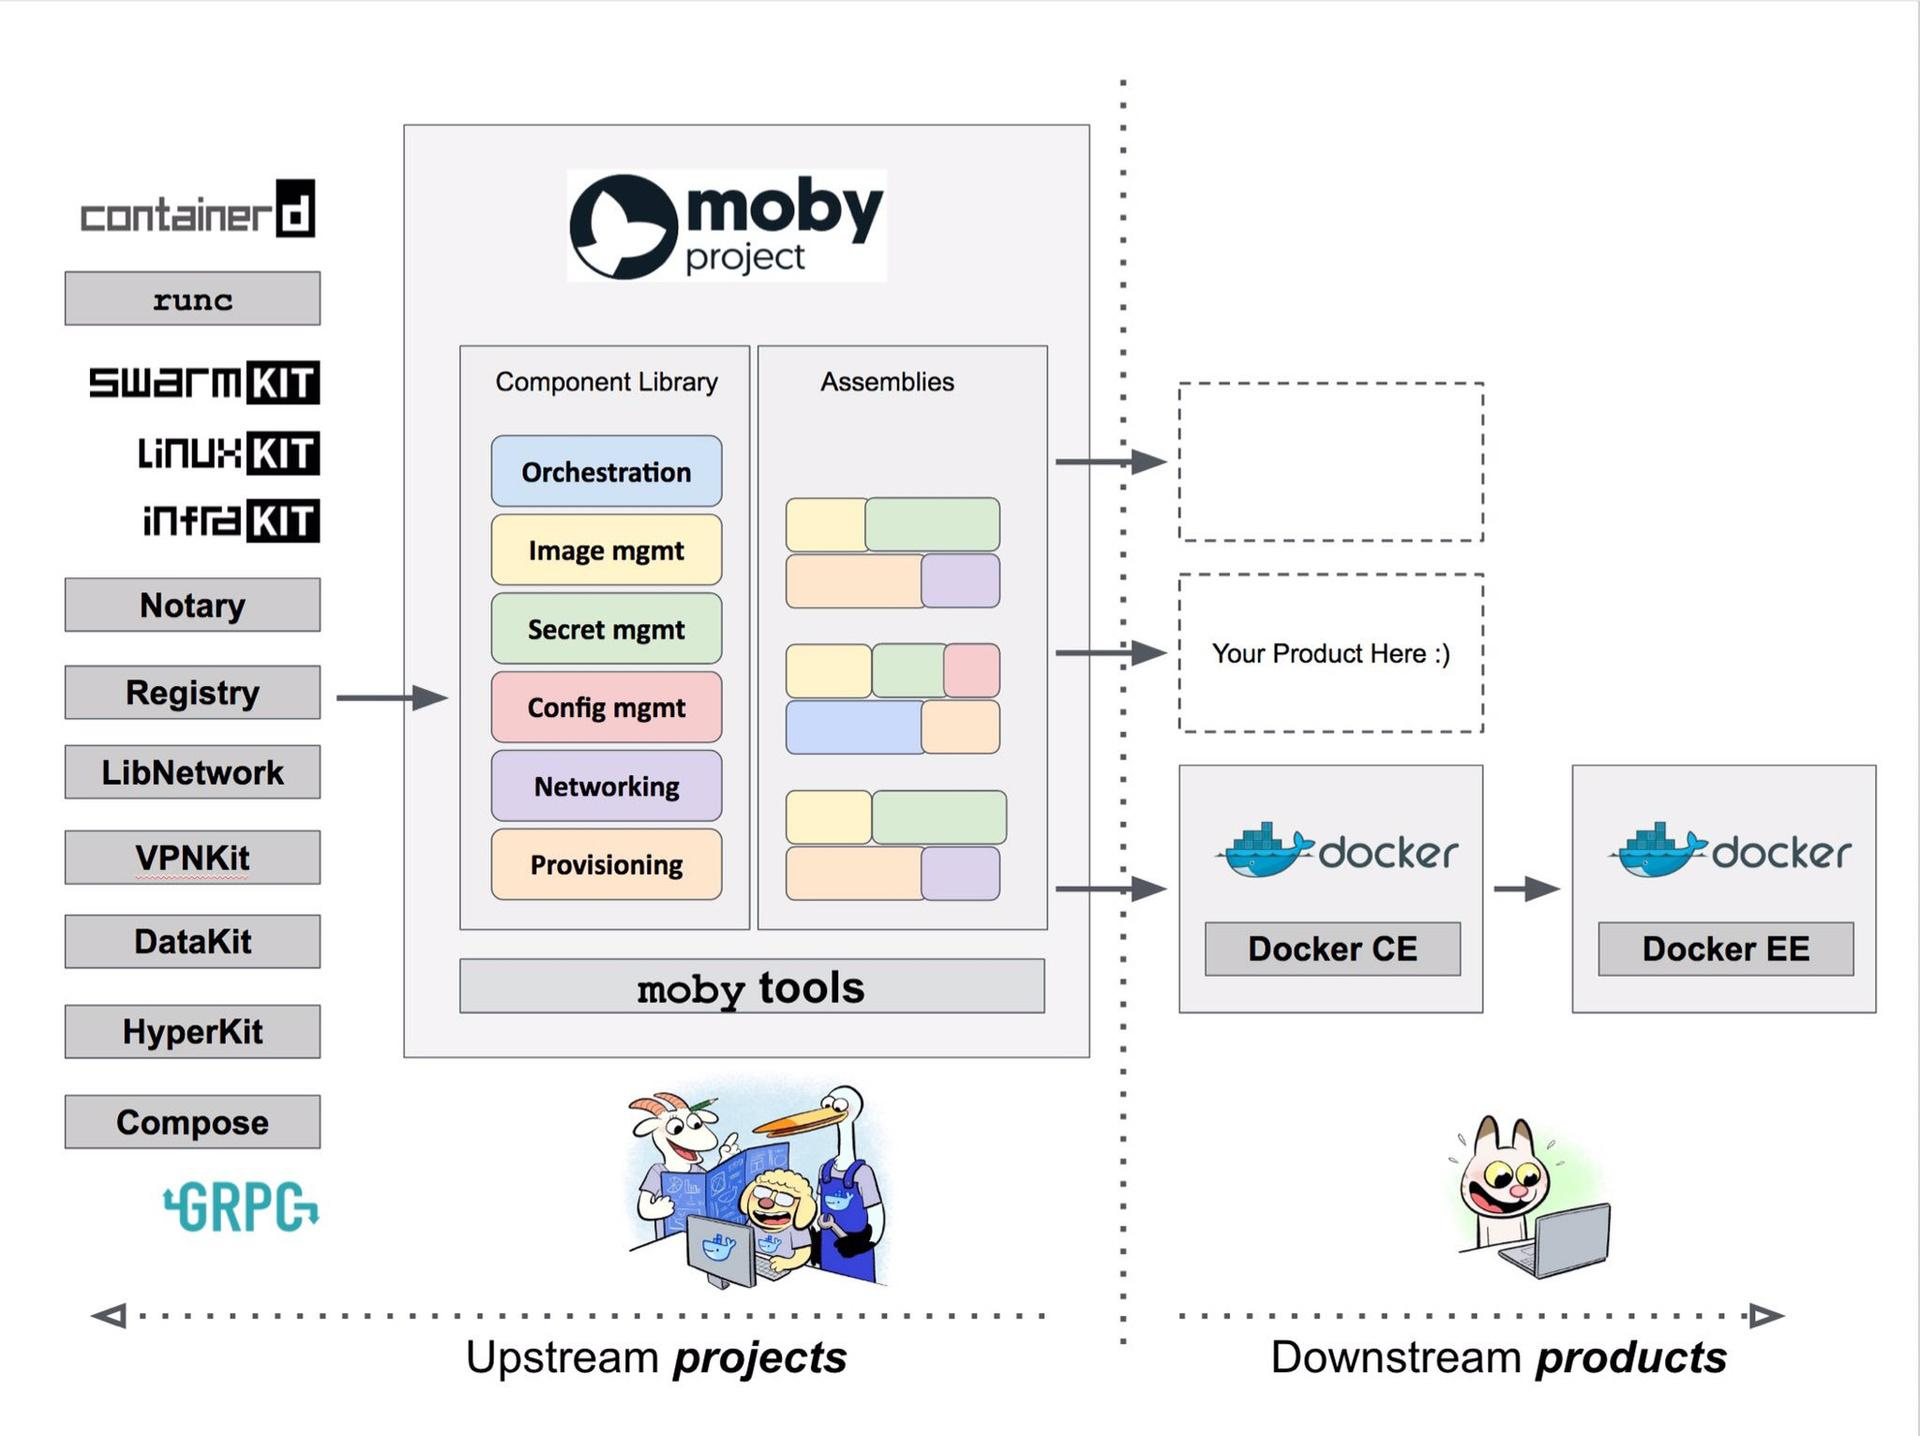
\includegraphics[width=1\textwidth]{imgs/3.2.jpg}}
    \label{3.2}
\end{figure}

Также стоит отметить, что модульность стала возможна благодаря стандартизации некоторых
компонентов в рамках проекта Linux Foundation под названием Open Container Initiative (OCI). В
частности, были разработаны \href{}{стандарты для среды исполнения} и \href{https://github.com/opencontainers/runtime-spec}{образов контейнеров}. Причём в
обоих случаях наработки Docker Inc. послужили основой для стандартов. Стоит упомянуть лишь runC,
который, будучи изначально частью Docker engine, претерпел небольшие изменения и стал базовой
реализацией среды выполнения контейнеров.

Фактически стандартизация формата образов и среды выполнения привела к тому, что появилась
возможность использовать одни и те же образы с самыми разнообразными средами запуска. Более
того, это дало толчок бурному развитию систем запуска контейнеров: \href{https://github.com/cri-o/cri-o}{CRI-O}, 
\href{https://github.com/rkt/rkt}{rkt}, \href{https://docs.microsoft.com/en-us/virtualization/windowscontainers/deploy-containers/containerd}{runhcs}, \href{https://github.com/kata-containers/runtime}{kata-runtime}.
Причём некоторые среды запуска вышли за пределы исходного определения контейнеров. Они
используют аппаратные средства ускорения виртуализации для создания более безопасных
окружений — легковесных виртуальных машин. Примеры таких окружений: Kata containers и
контейнеры Windows при использовании Hyper-V изоляции. Не путайте с Docker-desktop, но об этом
позднее.

Возвращаясь к Docker, поговорим о его особенностях по сравнению с ранее рассмотренными
Virtuozzo/OpenVZ и LXC.\\

\subsubsection*{Контейнер приложения}
\addcontentsline{toc}{subsubsection}{Контейнер приложения}

Важное отличие от ранее существовавших систем контейнеризации — смещение фокуса с эмуляции
полноценной системы к легковесному контейнеру, содержащему только одно приложение и все
требующиеся ему зависимости. Если использовать контейнер не как альтернативу виртуальной
машине у хостинг-провайдера, а как способ упаковки одного сервиса или приложения с необходимым
окружением, то можно выкинуть из такого контейнера всё лишнее. Можно сократить объём памяти,
занимаемый контейнером и его образом, и использование ресурсов процессора за счёт исключения
запуска служебных процессов: разнообразных демонов и даже системы инициализации.

\begin{figure}[H]
    \centering
    \scalebox{0.9}{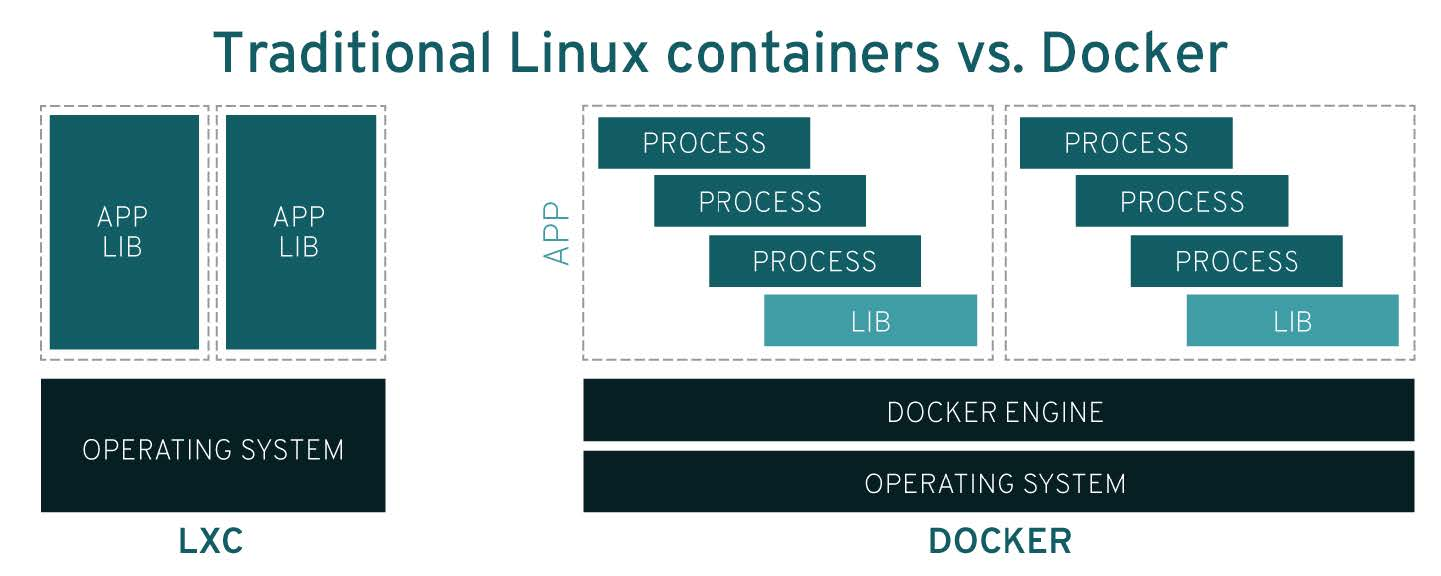
\includegraphics[width=1\textwidth]{imgs/3.3.jpg}}
    \caption*{\textit{Read Hat \href{https://www.redhat.com/en/topics/containers/what-is-docker}{Containers: What is DOCKER?}\\}}
    \label{3.3}
\end{figure}

\subsubsection*{Многослойные образы контейнеров}
\addcontentsline{toc}{subsubsection}{Многослойные образы контейнеров}

\begin{figure}[H]
    \centering
    \scalebox{0.7}{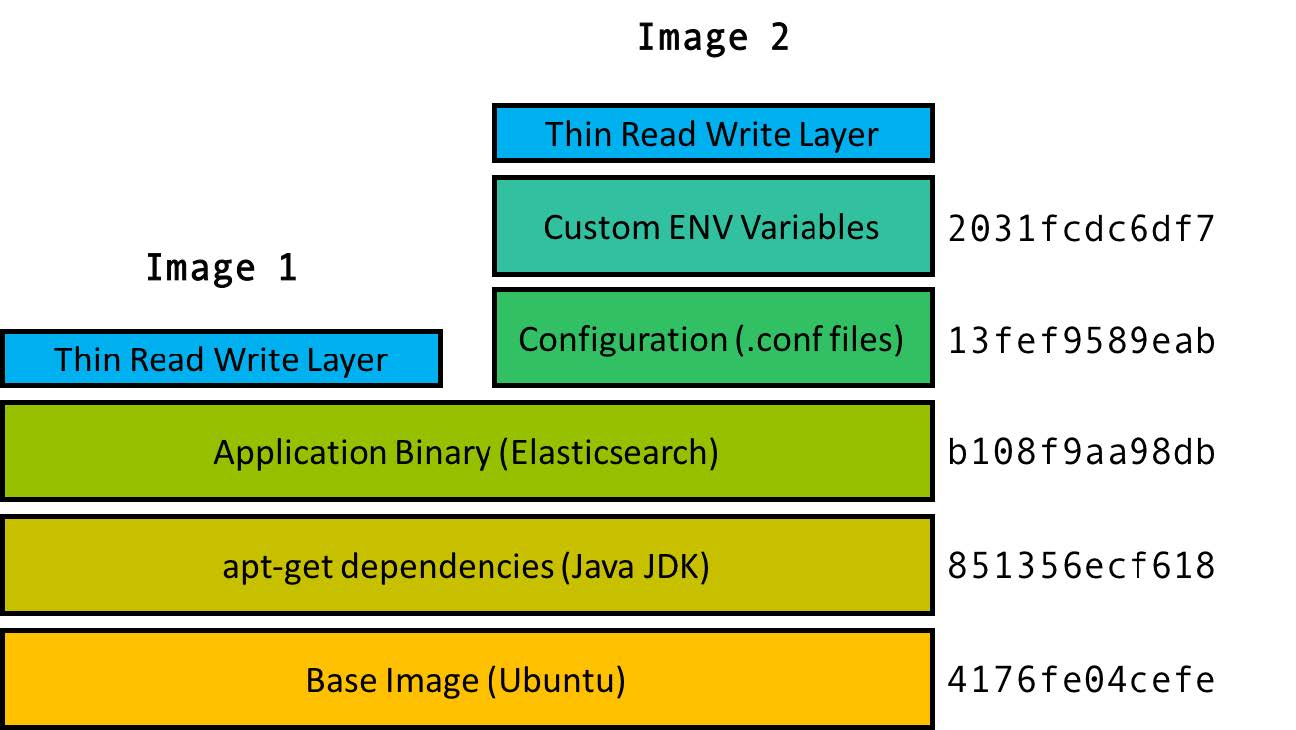
\includegraphics[width=1\textwidth]{imgs/3.4.jpg}}
    \caption*{\textit{\href{https://medium.com/nuances-of-programming/контейнеры-это-просто-контейнерные-технологии-для-начинающих-3912870fbc69}{Слои Docker}}}
    \label{3.4}
\end{figure}

Второе важное отличие — это многослойность. Преимущество перед монолитными образами состоит
в том, что теперь каждый из слоёв можно многократно использовать в других, более сложных,
образах. Безусловно, базовый образ — это, как правило, минималистичная файловая система
какого-то из популярных Linux-дистрибутивов, и она весьма монолитна. Но и то не совсем:
\begin{lstlisting}
$ docker history ubuntu:bionic
IMAGE           CREATED       CREATED BY SIZE
549b9b86cb8d    10 days ago   /bin/sh -c #(nop)  CMD ["/bin/bash"] 0B
<missing>       10 days ago   /bin/sh -c mkdir -p /run/systemd && echo 'do... 7B
<missing>       10 days ago   /bin/sh -c set -xe   && echo '#!/bin/sh' > /... 745B
<missing>       10 days ago   /bin/sh -c [ -z "$(apt-get indextargets)" ] 987kB
<missing>       10 days ago   /bin/sh -c #(nop) ADD file:53f100793e6c0adfc... 63.2MB 
\end{lstlisting}

Для сравнения, вот так выглядит более сложный образ \href{https://github.com/phusion/baseimage-docker}{Baseimage-docker}:
\begin{lstlisting}
$ docker history 166cfc3f6974
IMAGE           CREATED         CREATED BY SIZE
166cfc3f6974    23 months ago   /bin/sh -c #(nop) CMD ["/sbin/my_init"] 0B
<missing>       23 months ago   /bin/sh -c #(nop) ENV DEBIAN_FRONTEND=telety... 0B
<missing>       23 months ago   /bin/sh -c /bd_build/prepare.sh &&  /bd_buil... 97.3MB
<missing>       23 months ago   /bin/sh -c #(nop) COPY dir:e7a5eda59d878c69c... 39.4kB
<missing>       23 months ago   /bin/sh -c #(nop) MAINTAINER Phusion <info@p... 0B
<missing>       23 months ago   /bin/sh -c #(nop)  CMD ["/bin/bash"] 0B
<missing>       23 months ago   /bin/sh -c mkdir -p /run/systemd && echo 'do... 7B
<missing>       23 months ago   /bin/sh -c sed -i 's/^#\s*\(deb.*universe\)$... 2.76kB
<missing>       23 months ago   /bin/sh -c rm -rf /var/lib/apt/lists/* 0B
<missing>       23 months ago   /bin/sh -c set -xe   && echo '#!/bin/sh' > /... 745B
<missing>       23 months ago   /bin/sh -c #(nop) ADD file:a3344b835ea6fdc56... 112MB
\end{lstlisting}

Легко заметить большое количество изменений по сравнению с базовым образом Ubuntu 18.04.

Новый слой автоматически создаётся при выполнении каждой команды Dockerfile при создании
образа. В частности, вот так создавался образ, рассмотренный выше:
\begin{lstlisting}[language=docker]
ARG BASE_IMAGE=ubuntu:18.04
FROM $BASE_IMAGE
MAINTAINER Phusion <info@phusion.nl>

ARG QEMU_ARCH
ADD x86_64_qemu-${QEMU_ARCH}-static.tar.gz /usr/bin 

COPY . /bd_build

RUN /bd_build/prepare.sh && \
    /bd_build/system_services.sh && \
    /bd_build/utilities.sh && \
    /bd_build/cleanup.sh

ENV DEBIAN_FRONTEND="teletype" \ 
    LANG="en_US.UTF-8" \ 
    LANGUAGE="en_US:en" \ 
    LC_ALL="en_US.UTF-8"

CMD ["/sbin/my_init"]
\end{lstlisting}

Другие образы могут использовать его как свой базовый образ и так далее. Причём данные каждого
образа хранятся на локальной файловой системе в единственном экземпляре. То есть при запуске
десяти контейнеров, использующих один и тот же образ, на хозяйской системе будет храниться и
использоваться только один экземпляр образа. Более того, если будет создан новый образ на основе
имеющегося базового, то на диске хозяйской системы будет дополнительно сохранена только разница
между базовым и новым образами. Полезно вспомнить, что сокращение объёма используемой памяти
конвертируется в существенное ускорение работы системы. Это происходит благодаря тому, что
большая часть данных может быть доступна в быстрой памяти, близкой к процессору: кешах
процессора или, на худой конец, в ОЗУ, а не только на диске или в сети.

\subsubsection*{Поддержка различных хозяйских ОС}
\addcontentsline{toc}{subsubsection}{Поддержка различных хозяйских ОС}

Как мы помним, Virtuozzo/OpenVZ и LXC (Linux Containers даже по определению) существовали только
на хозяйских системах с ядром Linux, то есть фактически только в Linux-дистрибутивах. Однако
компания Docker Inc. сумела преодолеть это ограничение.

Первая возможность использовать Docker поверх хозяйской ОС, отличной от Linux-дистрибутива,
появилась благодаря использованию полноценной виртуальной машины, внутри которой был
запущен, собственно, Linux-дистрибутив. Справедливости ради отметим, что такой подход был
применим и к другим системам контейнеризации: любой желающий мог установить в виртуальной
машине Linux-дистрибутив и в нём Docker.

Такой подход не слишком удобен, так как не позволяет управлять системой контейнеризации
непосредственно из хозяйской системы. Все действия нужно производить, находясь внутри
виртуальной машины. То же касается сложностей со взаимодействием с сервисами или
приложениями внутри контейнеров: пользователю самому пришлось бы заниматься настройкой
проброса портов из хозяйской системы в гостевую и т. д.

Компания Docker в своём решении \href{https://docs.docker.com/toolbox/toolbox_install_windows/}{Docker Toolbox on Windows} (равно как и \href{https://docs.docker.com/toolbox/toolbox_install_mac/}{on Mac}) сделала работу с
контейнерами в виртуальной машине гораздо более удобной. Она предложила настроить всё за
пользователя и предоставила удобный инструментарий специально для такого сценария:

\begin{enumerate}
    \item \href{https://kitematic.com/}{Kinematic} — графическая утилита для управления контейнерами.
    \item \href{https://docs.docker.com/machine/overview/}{Docker Machine} — утилита командной строки для управления виртуальными окружениями и
    контейнерами в них.
    \item Docker Quickstart — терминал, настроенный для работы с Docker Engine внутри виртуальной
    машины.
    \item Виртуальная машина для Oracle VirtualBox с установленным легковесным
    Linux-дистрибутивом Boot2Docker.
\end{enumerate}

\href{https://github.com/boot2docker/boot2docker}{Boot2Docker} — легковесный Linux-дистрибутив, созданный на базе \href{http://tinycorelinux.net/}{Tiny Core Linux}. Работает будучи
полностью загруженным в ОЗУ, имеет загружаемый образ размером ~45 Мбайт. В настоящее время
находится в режиме минимальной поддержки как запасной вариант для пользователей, которые по
разным причинам не могут использовать более современное решение Docker for Windows или Docker
for Mac. Это пользователи Windows 7, для которой Docker for Windows просто недоступен, и
пользователи Windows 10 Home, в которой невозможно включить Microsoft Hyper-V.

Благодаря этим нововведениям значительно улучшился пользовательский опыт при работе с
контейнерами из Windows или macOS. На это решение был высокий спрос, но его эффективность
была низкой из-за необходимости запуска полноценной виртуальной машины, причём «чужой» для
хозяйской ОС. В качестве виртуальной машины использовался Oracle VirtualBox — решение хоть и
доступное на Windows и macOS, но тем не менее не очень интегрированное в хозяйскую ОС. Другого
и нельзя было ожидать от продукта стороннего относительно хозяйской ОС производителя.

В результате миру были представлены более интегрированные с хозяйской ОС решения: \href{https://docs.docker.com/docker-for-windows/}{Docker
Desktop for Windows} и \href{https://docs.docker.com/docker-for-mac/}{Docker Desktop for Mac}.


\paragraph*{Docker for Windows} \mbox{}\\
\addcontentsline{toc}{paragraph}{Docker for Windows}

В Docker for Windows для запуска \href{https://docs.microsoft.com/en-us/virtualization/windowscontainers/deploy-containers/linux-containers}{Linux-контейнеров} используется встроенный гипервизор Microsoft
Hyper-V. Под его управлением запускается минималистичная, хотя всё ещё полноценная, виртуальная
машина со специально подготовленным Linux-дистрибутивом. Это собранный при помощи LinuxKit
дистрибутив, что можно засвидетельствовать, обнаружив работающей виртуальную машину
DockerDesktopVM.

\begin{lstlisting}[basicstyle=\fontsize{8}{13}\selectfont\ttfamily, numberstyle=\color{152, 104, 1}]
PS C:\> Get-VM

Name            State   CPUUsage(%)  MemoryAssigned(M)  Uptime     Status           Version
----            -----   -----------  -----------------  ------     ------           -------
DockerDesktopVM Running 0            2048               00:01:14   Работает нормально  9.0

\end{lstlisting}

\href{https://github.com/linuxkit/linuxkit}{LinuxKit} — инструмент построения Linux-дистрибутивов, специально предназначенных для запуска
систем контейнеризации.

Похоже, что до настоящего времени инженеры Docker Inc. не могут решить, как называть виртуальную
машину. До сих пор мы видели Moby VM, MobyLinuxVM и DockerDesktopVM.

В отличие от более ранней реализации Docker Toolbox for Windows, в Docker Desktop for Windows
часть инструментария запускается непосредственно в хозяйской ОС Windows. В случае
использования полноценной виртуальной машины это клиент Docker (собственно, утилита docker).
Тем не менее одна и та же виртуальная машина используется для запуска всех контейнеров, то есть
все они используют одно и то же ядро Linux. Более того, поскольку Docker Engine находится внутри
той же виртуальной машины, её приходится всё время держать включённой, иначе не удастся
запустить контейнер в случае необходимости.


\begin{figure}[H]
    \centering
    \scalebox{0.7}{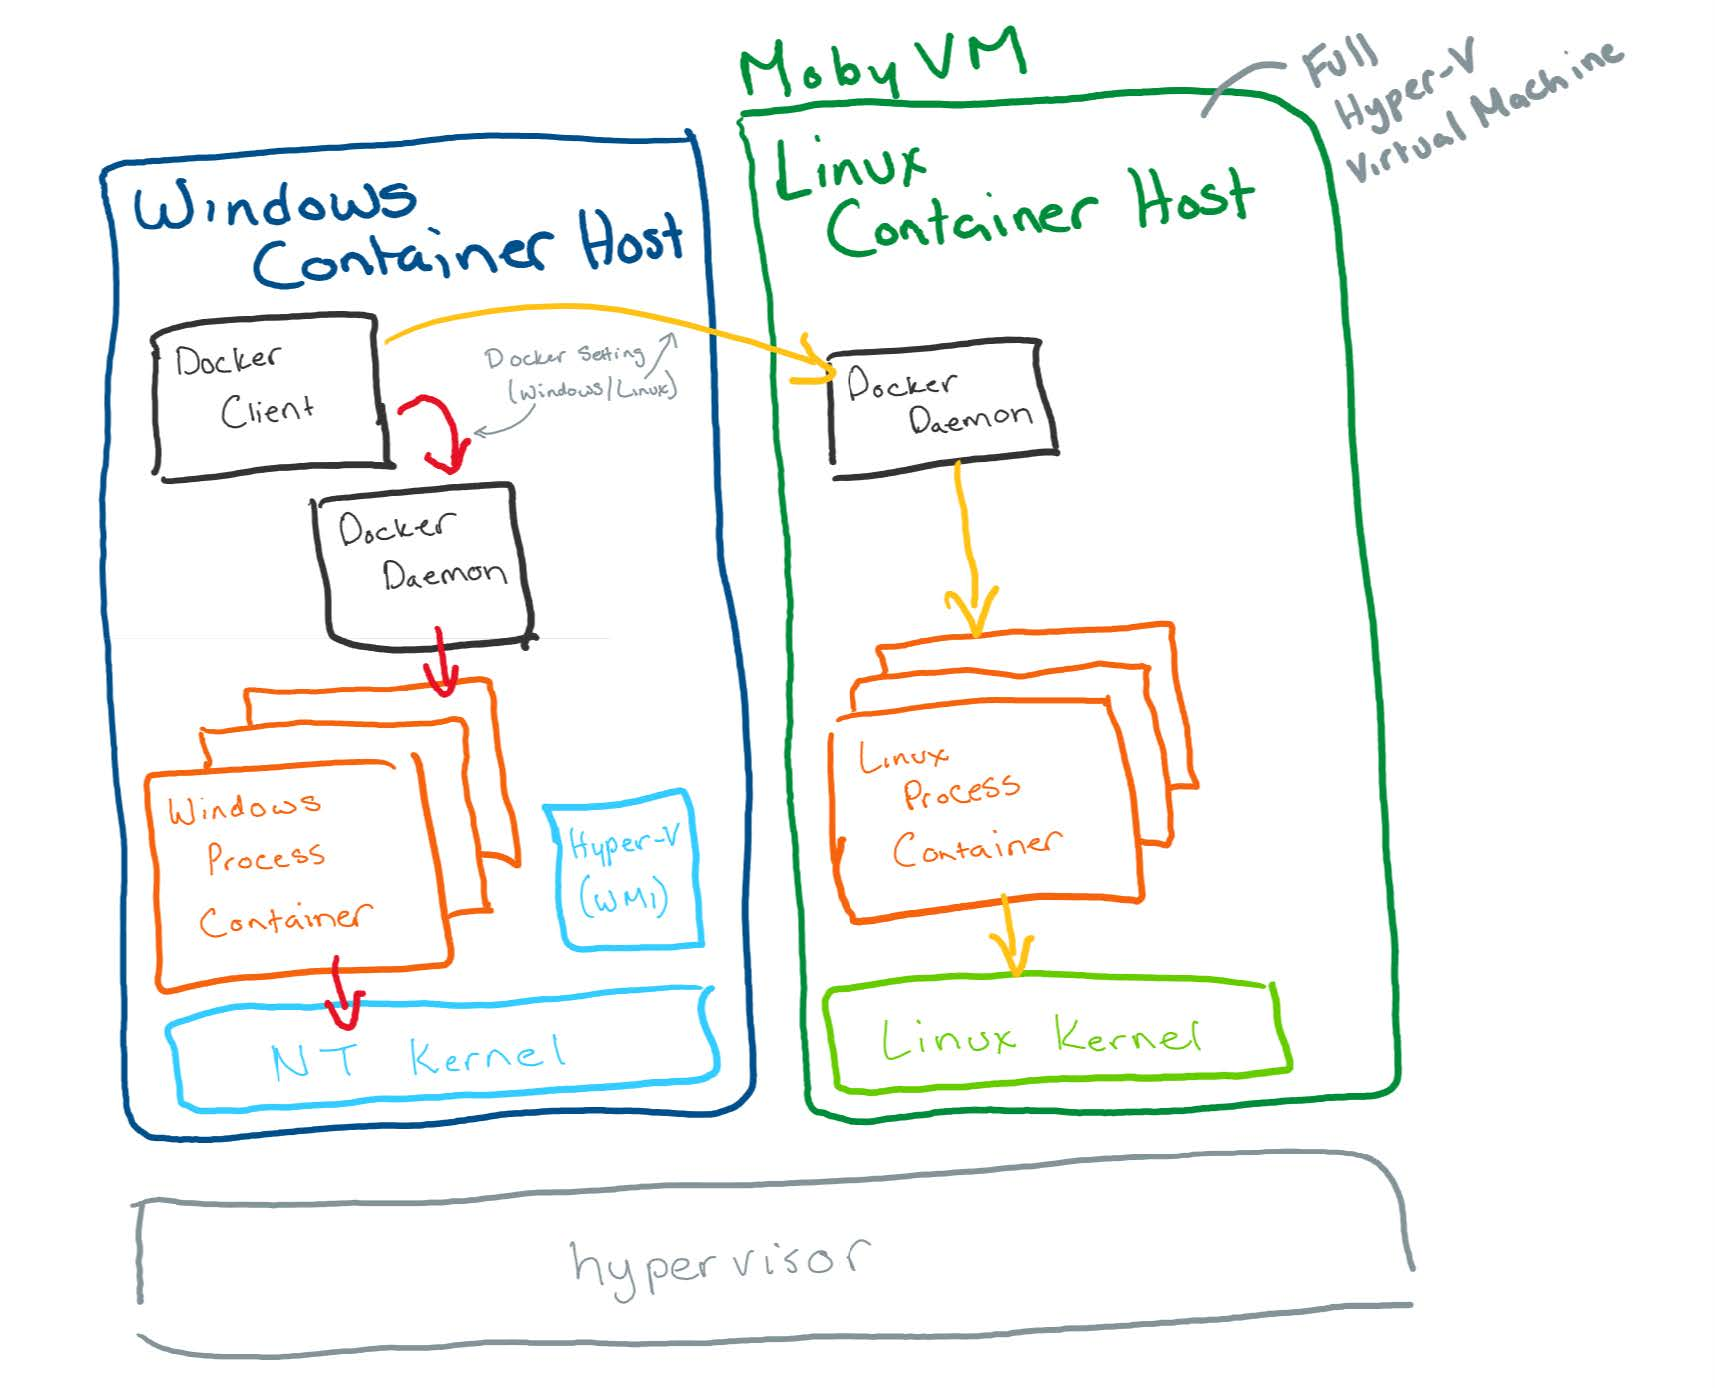
\includegraphics[width=1\textwidth]{imgs/3.5.jpg}}
    \caption*{\textit{\href{https://docs.microsoft.com/en-us/virtualization/windowscontainers/deploy-containers/linux-containers}{Устройство Docker for Windows с полноценной виртуальной машиной}}}
    \label{3.5}
\end{figure}

Сейчас ведётся активная работа над новой реализацией Linux-контейнеров в Windows c названием
LCOW (Linux Containers on Windows). Её существенные отличия: во-первых, каждый контейнер
запускается в собственном виртуальном окружении и использует свою собственную копию ядра Linux,
а во-вторых, всё управление контейнерами происходит на стороне хозяйской ОС. В том числе и
Docker Engine остаётся в хозяйской системе, а виртуальные окружения создаются по запросу при
необходимости. Интересно, что такие виртуальные окружения не видны в диспетчере Hyper-V, даже
когда Linux-контейнер запущен на исполнение.

Для примера можно запустить новый контейнер с Ubuntu 18.04:

\begin{lstlisting}
PS C:\> docker run --rm -i -t ubuntu bash
root@bf2f16d5b75b:/# uname -a
Linux bf2f16d5b75b 4.19.27-linuxkit #1 SMP Sun Mar 10 18:51:44 UTC 2019 x86_64 x86_64 x86_64 
GNU/Linux
root@bf2f16d5b75b:/# cat /etc/issue
Ubuntu 18.04.3 LTS \n \l
\end{lstlisting}

И попытаться обнаружить запущенную виртуальную машину:

\begin{lstlisting}[basicstyle=\fontsize{8}{13}\selectfont\ttfamily, numberstyle=\color{152, 104, 1}]
PS C:\> Get-VM
Name             State  CPUUsage(%) MemoryAssigned(M) Uptime   Status             Version
----             -----  ----------- ----------------- ------   ------             -------
DockerDesktopVM  Off    0           0                 00:00:00 Работает нормально    9.0
\end{lstlisting}

Утилита Get-VM ожидаемо рапортует о наличии лишь остановленной виртуальной машины, которая
использовалась ранее при запуске Linux-контейнера без LCOW. Зато при помощи утилит
\href{https://docs.microsoft.com/en-us/powershell/module/hostcomputeservice/get-computeprocess}{Get-ComputeProcess} и hcsdiag можно обнаружить наш контейнер. Смотрите объект с Id, совпадающим
с Id Docker-контейнера:

\begin{lstlisting}
PS C:\> Get-ComputeProcess
RunspaceId        : f43e60a7-8e89-4a49-8c72-20295e060568 
Id                : 9BE2B7E6-8724-4A60-A55B-DFF189F1919A
Type              : VirtualMachine
Isolation         : VirtualMachine
IsTemplate        : False
RuntimeId         : 9be2b7e6-8724-4a60-a55b-dff189f1919a 
RuntimeTemplateId :
RuntimeImagePath  : 
Owner             : VMMS

RunspaceId        : f43e60a7-8e89-4a49-8c72-20295e060568 
Id                : bf2f16d5b75b351b7dfeb42c16f56741c35e2f442ccf287f2bbece4f587cbc93 
Type              : Container
Isolation         : HyperV
IsTemplate        : False
RuntimeId         : cf4d055f-e68b-4f62-8f44-90ca03e9d592 
RuntimeTemplateId :
RuntimeImagePath  : C:\Program Files\Linux Containers 
Owner             : docker

PS C:\> hcsdiag list
9BE2B7E6-8724-4A60-A55B-DFF189F1919A
VM, Created, 9BE2B7E6-8724-4A60-A55B-DFF189F1919A,
VMMS

bf2f16d5b75b351b7dfeb42c16f56741c35e2f442ccf287f2bbece4f587cbc93
Hyper-V Linux Container, Running, CF4D055F-E68B-4F62-8F44-90CA03E9D592,
docker
\end{lstlisting}

\begin{figure}[H]
    \centering
    \scalebox{0.7}{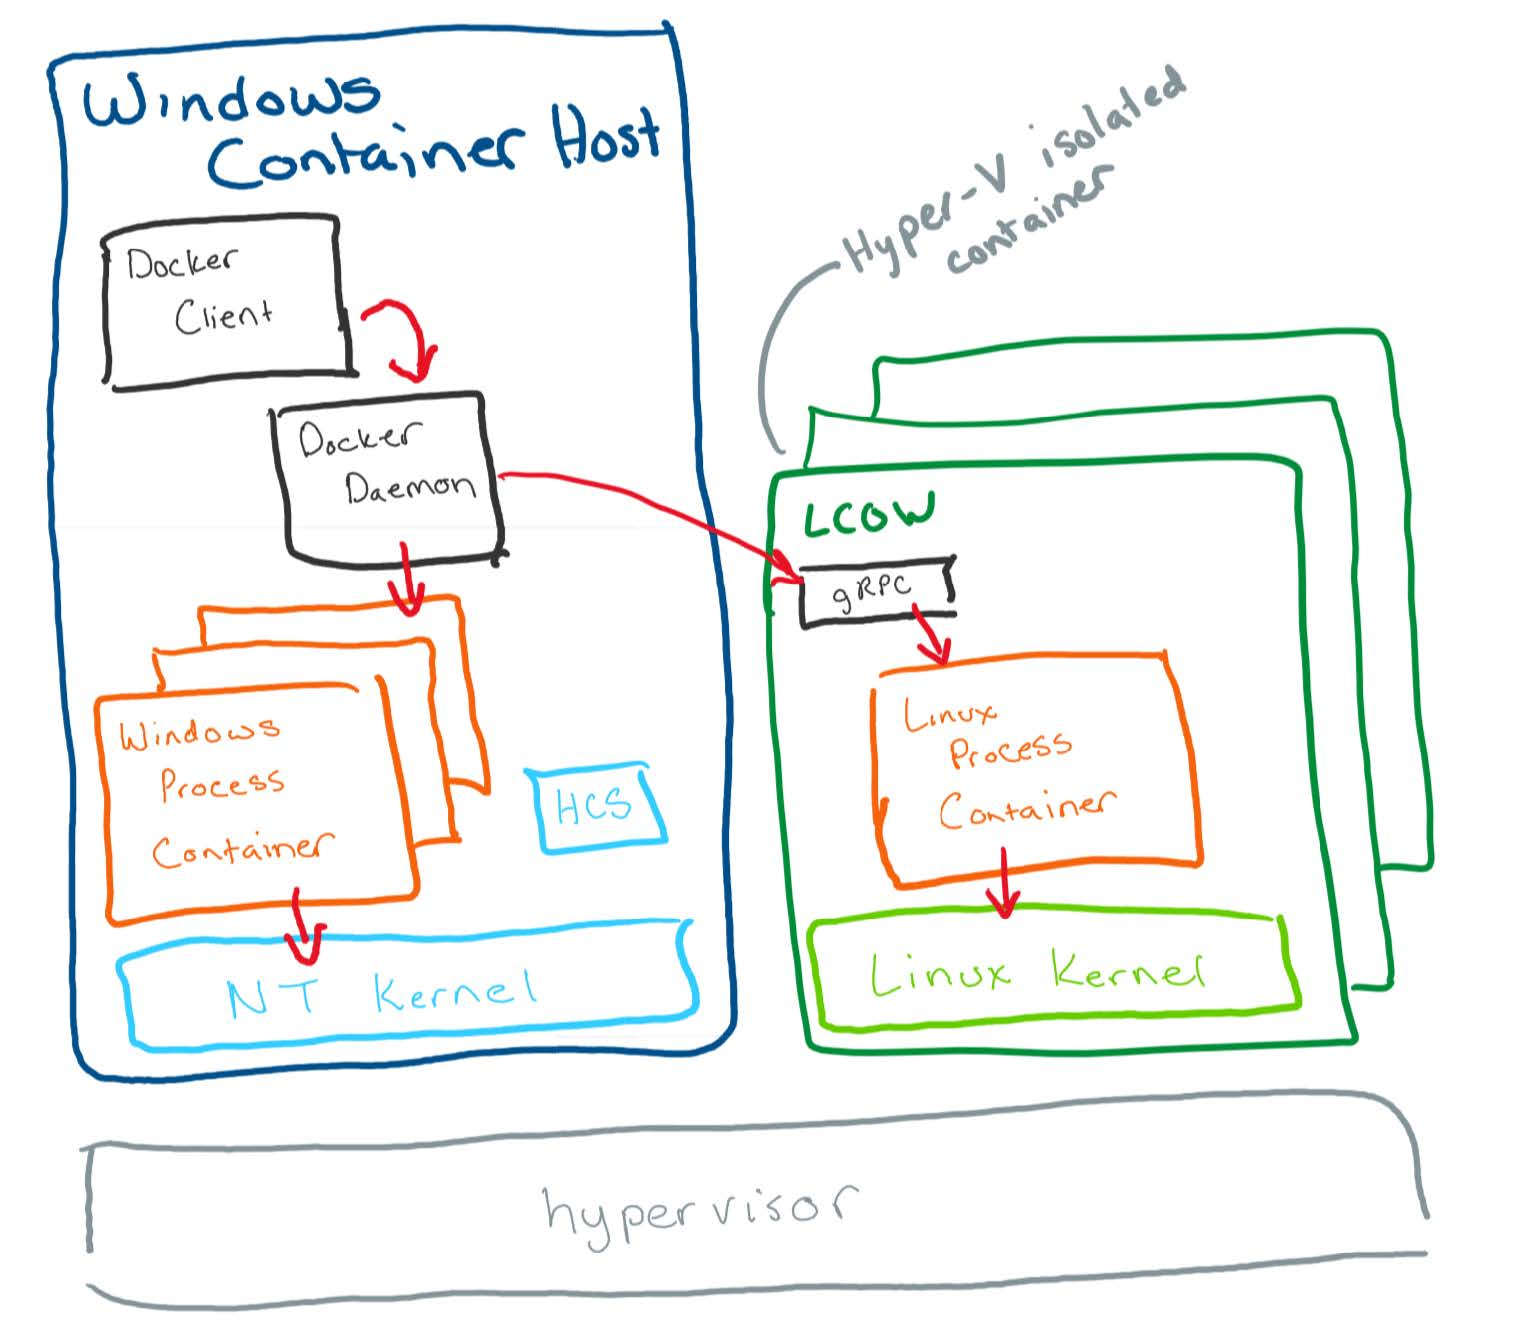
\includegraphics[width=1\textwidth]{imgs/3.6.jpg}}
    \caption*{\textit{\href{https://docs.microsoft.com/en-us/virtualization/windowscontainers/deploy-containers/linux-containers}{Устройство Docker for Windows с LCOW}}}
    \label{3.6}
\end{figure}

Интересно заметить, что реализация LCOW стала возможной благодаря ранее проделанной над
Windows-контейнерами работе. \href{https://azure.microsoft.com/ru-ru/blog/containers-docker-windows-and-trends/}{Разработка Windows-контейнеров} велась совместными усилиями
инженеров Microsoft и Docker Inc. Одним из результатов работы над Windows Server Containers стал
метод изоляции при помощи гипервизора Microsoft Hyper-V, который затем был использован для
запуска Linux-контейнеров в легковесных виртуальных окружениях \href{https://docs.microsoft.com/en-us/virtualization/community/team-blog/2017/20170127-introducing-the-host-compute-service-hcs}{Host Compute Service (HCS)}.

Ещё одно преимущество использования LCOW — возможность одновременного запуска Linux- и
Windows-контейнеров. Это наглядно представлено примером ниже:

\begin{lstlisting}
PS C:\> docker run -d -p 8080:8080 --isolation=process chocolateyfest/appetizer:1.0.0 
8c18315559fc8aab0c67723c12fa6666ba224f738c8f65ab2028f64f6caebaf6

PS C:\> start http://localhost:8080

PS C:\> docker container ls
CONTAINER ID IMAGE                         COMMAND       CREATED        STATUS PORTS             NAMES
8c18315559fc chocolateyfest/appetizer:1.0.0 "node app.js" 37 seconds ago Up 37 seconds 0.0.0.0:8080->8080/tcp   eager_faraday bf2f16d5b75b ubuntu "bash" 32 minutes ago Up 32 minutes  clever_brown

\end{lstlisting}

\begin{figure}[H]
    \centering
    \scalebox{1}{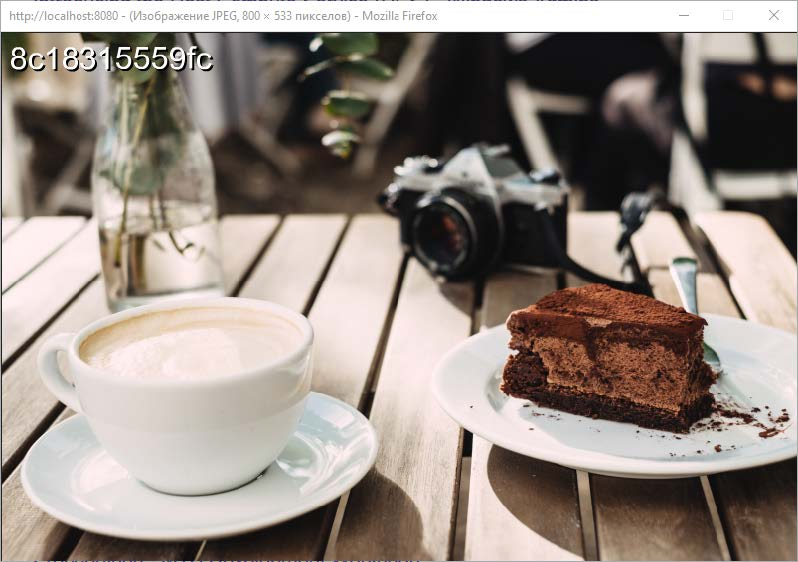
\includegraphics[width=1\textwidth]{imgs/3.7.jpg}}
    \label{3.7}
\end{figure}

В заключение разговора о Docker на Windows хочется заметить, что после удачного старта
Windows-контейнеров на базе Docker инженеры Microsoft начали работы по выделению среды запуска
контейнеров в независимый внешний компонент. Так появился \href{https://docs.microsoft.com/en-us/virtualization/windowscontainers/deploy-containers/containerd#runhcs}{runhcs}. По сути, runhcs — это
видоизмененный \href{https://github.com/microsoft/hcsshim/tree/master/cmd/runhcs}{runC} для работы в Windows и запуска контейнеров при помощи HCS. Это открывает
дорогу на платформу Windows для других высокоуровневых систем управления контейнерами.\\

\paragraph*{Docker for Mac} \mbox{}\\
\addcontentsline{toc}{paragraph}{Docker for Mac}

Docker for Mac использует подход с запуском Linux-дистрибутива, построенного при помощи LinuxKit
под управлением \href{https://github.com/moby/hyperkit}{гипервизора HyperKit}, который разработали инженеры Docker Inc специально для
работы с Docker. По сути, это мало чем отличается от Docker for Windows с MobyVM, то есть без
использования LCOW. Весь Docker Engine и все контейнеры запускаются в одной перманентно
запущенной виртуальной машине, что определённо не слишком удобно.

Существенное отличие Docker for Mac от Docker for Windows состоит в том, что на сегодняшний день
не существует Mac-контейнеров. То есть на Mac возможно использование только Linux-контейнеров.

Однако стоит иметь в виду, что использование контейнеров в неродном окружении, то есть не в
Linux-дистрибутиве, являющемся хозяйской ОС, чревато шероховатостями: более низкой
эффективностью использования вычислительных ресурсов системы, \href{https://github.com/docker/for-mac/issues/77}{существенным снижением
скорости работы контейнеризованных приложений} и т. д. То есть использование систем с Windows
или macOS для «боевого» запуска приложения в контейнерах не имеет смысла. Тем не менее Docker
for Windows/Mac даёт возможность заниматься разработкой, связанной с использованием
контейнеров, в привычном для инженера окружении.\\


\paragraph*{Docker: заключение} \mbox{}\\
\addcontentsline{toc}{paragraph}{Docker: заключение}

Мы поговорили об инструментах, разработанных компанией Docker Inc. Всё началось с использования
доступного к тому моменту инструментария Linux Containers (LXC). Затем случилась первая
существенная переработка Docker Engine с целью более эффективного решения новой задачи —
контейнеризации одного приложения или службы в противовес полной ОС. Следующая существенная
переработка Docker Engine привела к разделению монолитного исполняемого файла на несколько
самодостаточных сущностей, каждая из которых решала свою конкретную задачу. Более того,
некоторые из них легли в основу стандартов, разработанных Open Container Initiative (OCI). А далее в
игру вступили другие разработчики и даже компании, такие как IBM, Red Hat (ныне поглощенная IBM),
Google и т. д. Используя стандартные компоненты, они стали строить всё более совершенные и
функциональные системы, использующие контейнеры.\\


\subsection*{После Docker}
\addcontentsline{toc}{subsection}{После Docker}

Можно смело сказать, что Docker Inc. создала современный рынок решений, связанных с
использованием контейнеризованных окружений. Однако, как это иногда случается, звёздный час
Docker Inc., похоже, остался в прошлом. Инициативу перехватили другие игроки, и будущее компании
Docker Inc вызывает всё больше вопросов. Такие выводы можно сделать, опираясь на следующие
факты:
\begin{enumerate}
    \item Компания Docker Inc. \href{https://www.cnbc.com/2019/09/27/docker-is-trying-to-raise-money-following-arrival-of-ceo-rob-bearden.html}{всё ещё не приносит дохода} и всецело зависит от внешних инвестиций.
    Исполнительный директор Docker Inc. в сентябре 2019 года разослал письмо сотрудникам о
    работе с двумя потенциальным инвесторами, которые могут обеспечить достаточное
    финансирование в будущем.
    \item Mirantis приобретает Docker Enterprise у Docker Inc.
    \item \href{http://crunchtools.com/docker-support/}{Red Hat отказалась от использования Docker} в OpenShift 4 и Red Hat Enterprise Linux 8 в
    пользу своей собственной разработки Podman/Buildah/Skopeo.
\end{enumerate}

Так что будем с интересом смотреть в будущее и наблюдать за рождением новых продуктов и
технологий если не от Docker Inc., то от кого-то другого.

Тем не менее именно благодаря Docker появились стандарты на образы контейнеров и сред их
выполнения. Это открыло дорогу к созданию инструментов для управления контейнерами на любой
вкус. Так появились:

\begin{itemize}
    \item CRI-O и Podman/Buildah/Skopeo от Red Hat как альтернатива управления контейнерами без
    демона dockerd;
    \item масса окружений для запуска контейнеров: \href{https://github.com/containers/crun}{crun}, \href{https://github.com/hyperhq/runv}{runv}, \href{https://github.com/Microsoft/hcsshim/tree/master/cmd/runhcs}{runhcs}.
\end{itemize}

crun — это runC, переписанный на языке Си.

runV — среда запуска контейнеров, использующая средства гипервизоров.

runhcs — порт runC для Microsoft Host Compute Services (HCS).

Так что стоит ожидать развития имеющихся и появления новых инструментов, каждый из которых
либо лучше решает уже знакомые задачи, либо нацелен на решение доселе неизвестных задач. Кто
бы мог подумать, что технологии, использующие базовые принципы и инструменты ОС с ядром Linux,
будут реализованы как родные на совершенно чужеродной платформе Windows!

На этой радостной ноте можно было бы закончить разговор о контейнерах, но хочется упомянуть ещё
один интересный феномен — использование средств аппаратной виртуализации для запуска
контейнеров.

\subsection*{Контейнеры в легковесных виртуальных машинах}
\addcontentsline{toc}{subsection}{Контейнеры в легковесных виртуальных машинах}

Ещё говоря о Docker for Windows, мы узнали, что запуск Windows-контейнеров может осуществляться
в одном из двух окружений:

\begin{itemize}
    \item с изоляцией процессов друг от друга средствами ОС (аналог идеи контейнеров в Linux);
    \item с изоляцией при помощи гипервизора Hyper-V (этот же режим используется LCOW).
\end{itemize}

Использование аппаратных средств поддержки виртуализации при изоляции разных окружений сулит
большую безопасность, если говорить о возможности процессов из одного окружения проникнуть в
другое. Хотя мы помним, что случается всякое. А спрос на такую более надёжную изоляцию
определённо существует: например, при использовании одного и того же физического сервера для
запуска контейнеров разных хозяев. А если есть спрос, то появится и предложение. О решении на
платформе Windows мы уже поговорили, но что-то очень похожее есть и для Linux-систем. И имя
этому решению — \href{https://katacontainers.io/}{Kata containers}.

\begin{figure}[h]
    \centering
    \scalebox{0.9}{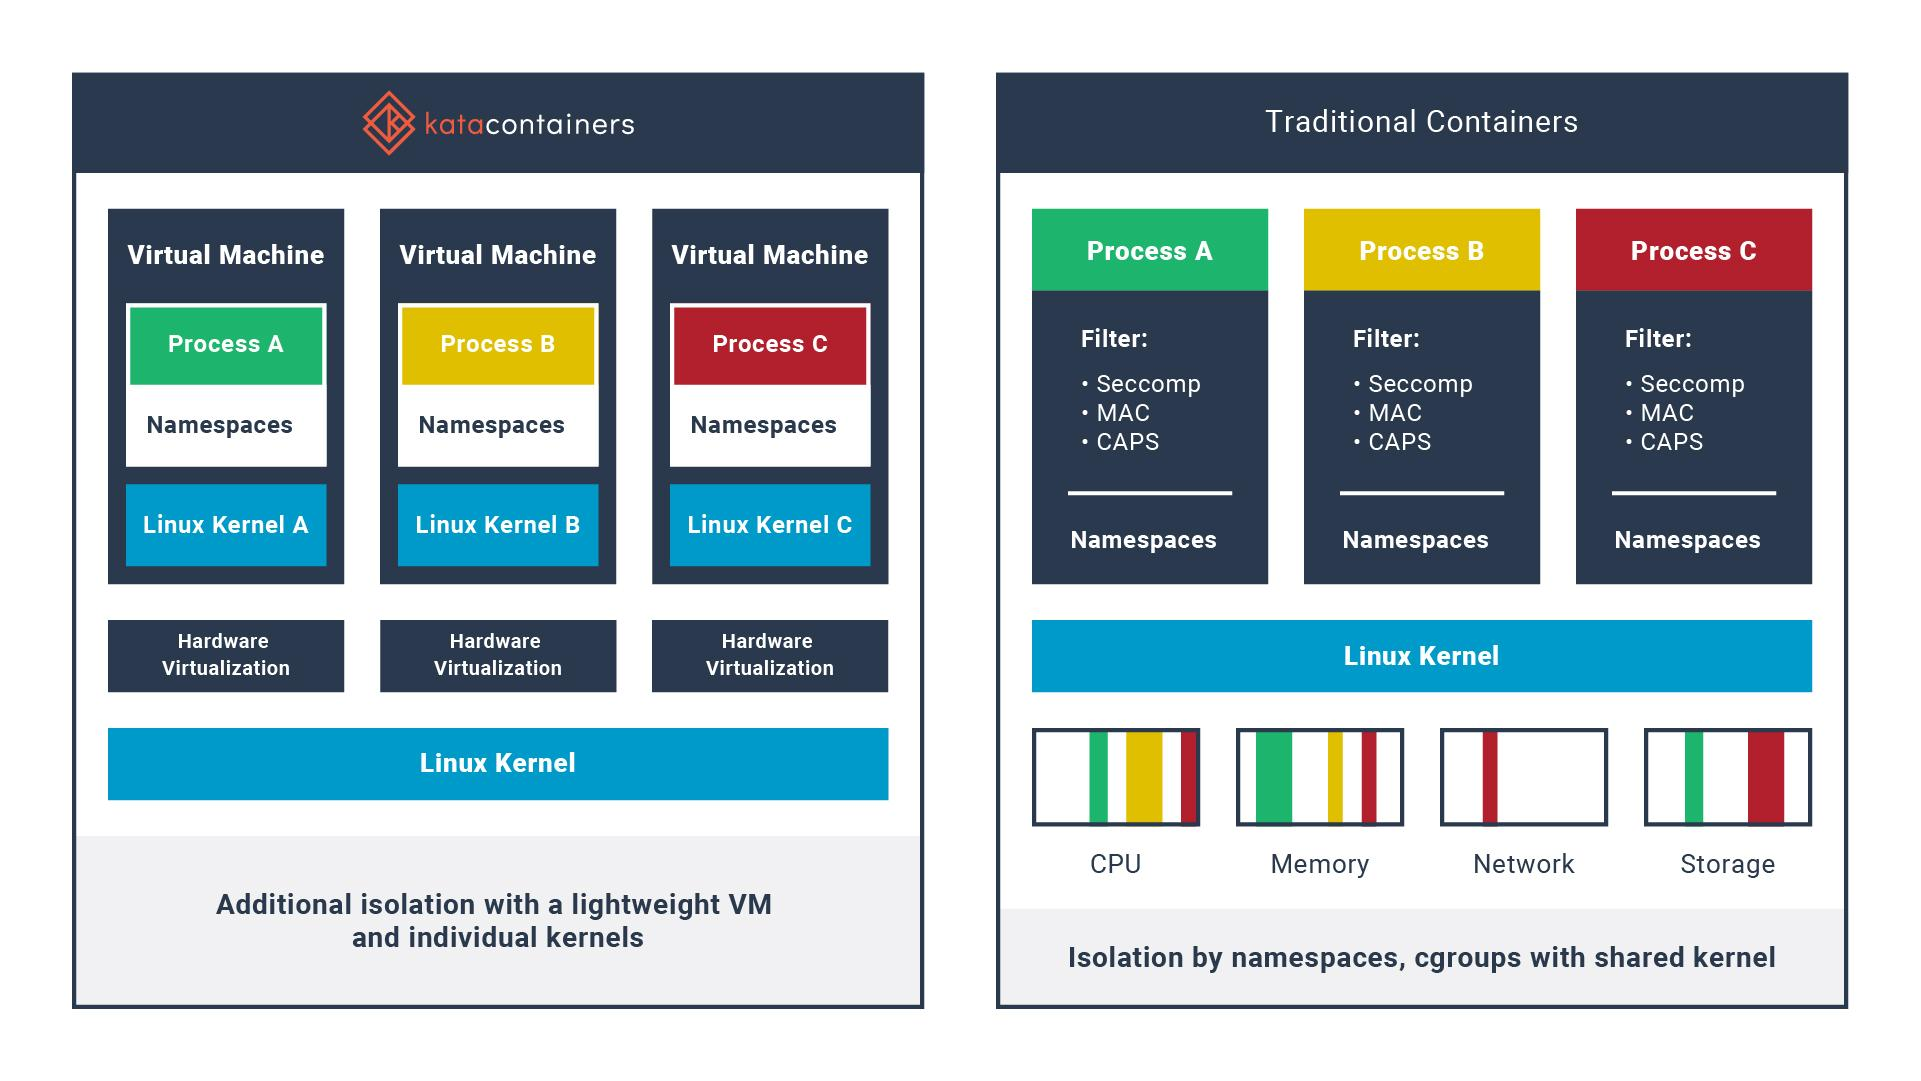
\includegraphics[width=1\textwidth]{imgs/3.8.jpg}}
    \caption*{\textit{Сравнение Kata Containers с обыкновенными контейнерами в Linux}}
    \label{3.8}
\end{figure}

Kata containers используют сильно оптимизированный Linux-дистрибутив, запущенный внутри
виртуальной машины. Поддержаны следующие гипервизоры: \href{https://projectacrn.org/}{ACRN}, \href{https://firecracker-microvm.github.io/}{QEMU/KVM}, \href{https://firecracker-microvm.github.io/}{Firecracker/KVM} и
\href{https://github.com/cloud-hypervisor/cloud-hypervisor}{Cloud Hypervisor/KVM}.

Кроме минимизации самого образа гостевой ОС, используются некоторые интересные оптимизации
как в ядре гостевой системы, так и на стороне гипервизора. Например, \href{https://www.kernel.org/doc/Documentation/filesystems/dax.txt}{DAX} — механизм доступа к
накопителю данных в обход страничного кеша. Также \href{https://ru.wikipedia.org/wiki/KSM}{KSM} (англ. kernel same-page merging, иногда
трактуется как kernel shared memory) — технология ядра Linux, которая позволяет ядру объединять
одинаковые страницы памяти между различными процессами или виртуальными гостевыми
системами в одну для совместного использования; реализация дедупликации данных для
оперативной памяти. Также для ускорения запуска контейнеров используются шаблоны виртуальных
машин.

Таким образом действительно достигается скорость запуска и работы контейнеризованных задач
намного выше, чем при ручном запуске контейнеров в обыкновенных виртуальных машинах. Более
того, плотность размещения Kata-контейнеров всё ещё гораздо ближе к таковой для обычных
контейнеров — много выше обыкновенных виртуальных машин.

А если прибавить соответствие стандарту OCI runtime и поддержку стандартных OCI-образов, то
получается действительно привлекательное решение. Его можно легко встроить в имеющуюся
инфраструктуру управления контейнерами, обеспечив при этом повышенную безопасность.\newpage


\section*{Заключение}
\addcontentsline{toc}{section}{Заключение}

Хотя контейнерная революция ещё даже не думает заканчиваться, мы можем наблюдать длинный и
интересный путь, проделанный системами управления контейнерами, начиная с Virtuozzo/OpenVZ и
заканчивая Cata containers. В недалёком будущем мы увидим новые интересные продукты,
технологии и даже области применения контейнеров вдобавок к тому, что мы имеем сегодня.

Можно смело констатировать, что контейнеры уже прочно вошли в жизнь многих инженеров,
компаний и даже индустрий. А потому стоит как минимум быть с ними знакомыми и готовыми к их
использованию.\newpage


\section*{Используемые источники}
\addcontentsline{toc}{section}{Используемые источники}

\begin{enumerate}
    \item \href{https://lwn.net/Articles/179361/}{Containers and lightweight virtualization.}
    \item \href{https://blog.selectel.ru/mexanizmy-kontejnerizacii-namespaces/}{Механизмы контейнеризации: namespaces.}
    \item \href{https://blog.selectel.ru/mexanizmy-kontejnerizacii-cgroups/}{Механизмы контейнеризации: cgroups.}
    \item \href{http://merrigrove.blogspot.com/2015/10/visualizing-docker-containers-and-images.html}{Visualizing Docker Containers and Images.}
    \href{https://habr.com/ru/post/272145/}{Перевод: Образы и контейнеры Docker в картинках.}
    \item \href{https://docs.microsoft.com/en-us/archive/msdn-magazine/2017/april/containers-bringing-docker-to-windows-developers-with-windows-server-containers}{Bringing Docker To Windows Developers with Windows Server Containers.}
    \item \href{https://medium.com/free-code-camp/comprehensive-introductory-guide-to-docker-vms-and-containers-4e42a13ee103}{A comprehensive introduction to Docker, Virtual Machines, and Containers.}
    \item \href{https://www.slideshare.net/PhilEstes/diving-through-the-layers-investigating-runc-containerd-and-the-docker-engine-architecture}{Diving Through The Layers: Investigating runc, containerd, and the Docker engine architecture.}
    \item \href{https://www.slideshare.net/nmeisenzahl/docker-meetup-rosenheim-container-runtimes}{Container Runtimes.}
    \item \href{https://habr.com/ru/post/272145/}{Образы и контейнеры Docker в картинках.}
    \item \href{https://medium.com/@waelkdouh/demystifying-docker-containers-support-on-windows-10-and-windows-server-2016-592f1c09a5e1}{Demystifying Docker Containers Support on Windows 10 and Windows Server 1709.}
    \item \href{http://collabnix.com/how-docker-for-mac-works-under-the-hood/}{Under the Hood: Demystifying Docker For Mac CE Edition.}
    \item \href{https://habr.com/ru/company/flant/blog/431192/}{В AWS представили Firecracker — «микровиртуализацию» для Linux.}
    \item \href{https://www.opennet.ru/opennews/art.shtml?num=51759}{Обновление гипервизоров Intel Cloud Hypervisor 0.3 и Amazon Firecracker 0.19, написанных на
    Rust.}
    \item \href{https://www.opennet.ru/opennews/art.shtml?num=51399}{Выпуск гипервизора для встраиваемых устройств ACRN 1.2, развиваемого в Linux Foundation.}
    \item \href{https://object-storage-ca-ymq-1.vexxhost.net/swift/v1/6e4619c416ff4bd19e1c087f27a43eea/www-assets-prod/presentation-media/Kata-Containers-The-way-to-run-virtualized-containers.pdf}{Kata Containers. The way to run virtualized containers.}
    \item \href{http://onreader.mdl.ru/ContainerizationWithLXC/content/index.html%20https://www.packtpub.com/virtualization-and-cloud/containerization-lxc}{Контейнеризация при помощи LXC.}
    \item \href{https://www.slideshare.net/Docker/windows-server-and-docker-the-internals-behind-bringing-docker-and-containers-to-windows-by-taylor-brown-and-john-starks}{Windows Server and Docker, The Internals Behind Bringing Docker and Containers to Windows.}
    \item \href{https://www.packtpub.com/virtualization-and-cloud/learning-windows-server-containers}{Learning Windows Server Containers.}\\
\end{enumerate}

\section*{Практическое задание}
\addcontentsline{toc}{section}{Практическое задание}

\begin{enumerate}
    \item Назовите преимущества и недостатки контейнеров по сравнению с виртуальными машинами.
    \item Запустите контейнер с базовым образом Ubuntu 18.04 в системе управления контейнерами на
    ваш выбор и выполните в запущенном контейнере несколько простых команд: uname, ls, cat.
    \item[3*.] Запустите систему управления контейнерами на ваш выбор внутри LXC-контейнера.
\end{enumerate}


\end{document}